\documentclass[oneside,numbers]{ezthesis}
%% # Opciones disponibles para el documento #
%%
%% Las opciones con un (*) son las opciones predeterminadas.
%%
%% Modo de compilar:
%%   draft            - borrador con marcas de fecha y sin im'agenes
%%   draftmarks       - borrador con marcas de fecha y con im'agenes
%%   final (*)        - version final de la tesis
%%
%% Tama'no de papel:
%%   letterpaper (*)  - tama'no carta (Am'erica)
%%   a4paper          - tama'no A4    (Europa)
%%
%% Formato de impresi'on:
%%   oneside          - hojas impresas por un solo lado
%%   twoside (*)      - hijas impresas por ambos lados
%%
%% Tama'no de letra:
%%   10pt, 11pt, o 12pt (*)
%%
%% Espaciado entre renglones:
%%   singlespace      - espacio sencillo
%%   onehalfspace (*) - espacio de 1.5
%%   doublespace      - a doble espacio
%%
%% Formato de las referencias bibliogr'aficas:
%%   numbers          - numeradas, p.e. [1]
%%   authoryear (*)   - por autor y a'no, p.e. (Newton, 1997)
%%
%% Opciones adicionales:
%%   spanish         - tesis escrita en espa'nol
%%
%% Desactivar opciones especiales:
%%   nobibtoc   - no incluir la bibiolgraf'ia en el 'Indice general
%%   nofancyhdr - no incluir "fancyhdr" para producir los encabezados
%%   nocolors   - no incluir "xcolor" para producir ligas con colores
%%   nographicx - no incluir "graphicx" para insertar gr'aficos
%%   nonatbib   - no incluir "natbib" para administrar la bibliograf'ia

%% Paquetes adicionales requeridos se pueden agregar tambi'en aqu'i.
%% Por ejemplo:
%\usepackage{subfig}
%\usepackage{multirow}
\usepackage{rotating,booktabs}
\usepackage{graphicx}
\graphicspath{{./img/}}
\DeclareGraphicsExtensions{.jpg,.png}
\usepackage{lscape}
\PassOptionsToPackage{USenglish}{babel}
\usepackage[USenglish]{babel} % espanol, ingles
\usepackage{multirow, array} %para mover el ancho de las tablas.
\renewcommand{\baselinestretch}{2}
\usepackage{vmargin}
\nocite{*}


\setpapersize{USletter}
\setmargins{3.2cm}       % margen izquierdo
{2.5cm}                        % margen superior
{15cm}                      % anchura del texto
{20cm}                    % altura del texto
{10pt}                           % altura de los encabezados
{1cm}                           % espacio entre el texto y los encabezados
{10pt}                             % altura del pie de página
{1cm}                           % espacio entre el texto y el pie de página

\usepackage{caption}
\usepackage{subfig}

\usepackage{amssymb, amsmath, amsbsy} % simbolitos
\usepackage{upgreek} % para poner letras griegas sin cursiva
\usepackage{cancel} % para tachar
\usepackage{mathdots} % para el comando \iddots
\usepackage{mathrsfs} % para formato de letra
\usepackage{stackrel} % para el comando \stackbin
\usepackage{enumerate} %para viñetas
%\usepackage{algpseudocode} %Para el apendice.
\usepackage{algorithm}
\usepackage{algorithmic}
\usepackage{listings}
%\usepackage{algpseudocode}
%\usepackage{pifont}

\usepackage[verbose]{placeins}
%\usepackage[ngerman]{babel}
\usepackage{blindtext}






%% # Datos del documento #
%% Nota que los acentos se deben escribir: \'a, \'e, \'i, etc.
%% La letra n con tilde es: \~n.

\author{Francisco Javier Arce C\'ardenas}
\title{Tesis Doctoral}
\degree{Doctor en Ciencias}
\supervisor{Jos\'e Mario Garc\'ia Valdez}
\institution{Instituto Tecnol\'ogico de Tijuana}
\faculty{Ciencias de la computac\'ion}
\department{Departamento de Sistemas Computacionales}

%% # M'argenes del documento #
%% 
%% Quitar el comentario en la siguiente linea para austar los m'argenes del
%% documento. Leer la documentaci'on de "geometry" para m'as informaci'on.

%\geometry{top=40mm,bottom=33mm,inner=40mm,outer=25mm}

%% El siguiente comando agrega ligas activas en el documento para las
%% referencias cruzadas y citas bibliogr'aficas. Tiene que ser *la 'ultima*
%% instrucci'on antes de \begin{document}.
\hyperlinking
\makeindex
\begin{document}
\pagenumbering{Roman}
%% En esta secci'on se describe la estructura del documento de la tesis.
%% Consulta los reglamentos de tu universidad para determinar el orden
%% y la cantidad de secciones que debes de incluir.

%% # Portada de la tesis #
%% Mirar el archivo "titlepage.tex" para los detalles.
%%% ## Construye tu propia portada ##
%% 
%% Una portada se conforma por una secuencia de "Blocks" que incluyen
%% piezas individuales de informaci'on. Un "Block" puede incluir, por
%% ejemplo, el t'itulo del documento, una im'agen (logotipo de la universidad),
%% el nombre del autor, nombre del supervisor, u cualquier otra pieza de
%% informaci'on.
%%
%% Cada "Block" aparece centrado horizontalmente en la p'agina y,
%% verticalmente, todos los "Blocks" se distruyen de manera uniforme 
%% a lo largo de p'agina.
%%
%% Nota tambi'en que, dentro de un mismo "Block" se pueden cortar
%% lineas usando el comando \\
%%
%% El tama'no del texto dentro de un "Block" se puede modificar usando uno de
%% los comandos:
%%   \small      \LARGE
%%   \large      \huge
%%   \Large      \Huge
%%
%% Y el tipo de letra se puede modificar usando:
%%   \bfseries - negritas
%%   \itshape  - it'alicas
%%   \scshape  - small caps
%%   \slshape  - slanted
%%   \sffamily - sans serif
%%
%% Para producir plantillas generales, la informaci'on que ha sido inclu'ida
%% en el archivo principal "tesis.tex" se puede accesar aqu'i usando:
%%   \insertauthor
%%   \inserttitle
%%   \insertsupervisor
%%   \insertinstitution
%%   \insertdegree
%%   \insertfaculty
%%   \insertdepartment
%%   \insertsubmitdate

\begin{titlepage}
  \TitleBlock{\scshape\insertinstitution}
  \TitleBlock[\bigskip]{\scshape\insertfaculty}
  \TitleBlock{\Huge\scshape\inserttitle}
  \TitleBlock{\scshape
    Tesis presentada por \insertauthor \\
    para obtener el grado de \insertdegree}
  \TitleBlock{\insertsubmitdate}
  \TitleBlock[\bigskip]{\insertdepartment}
\end{titlepage}

%% Nota 1:
%% Se puede agregar un escudo o logotipo en un "Block" como:
%%   \TitleBlock{\includegraphics[height=4cm]{escudo_uni}}
%% y teniendo un archivo "escudo_uni.pdf", "escudo_uni.png" o "escudo_uni.jpg"
%% en alg'un lugar donde LaTeX lo pueda encontrar.

%% Nota 2:
%% Normalmente, el espacio entre "Blocks" se extiende de modo que el
%% contenido se reparte uniformemente sobre toda la p'agina. Este
%% comportamiento se puede modificar para mantener fijo, por ejemplo, el
%% espacio entre un par de "Blocks". Escribiendo:
%%   \TitleBlock{Bloque 1}
%%   \TitleBlock[\bigskip]{Bloque2}
%% se deja un espacio "grande" y de tama~no fijo entre el bloque 1 y 2.
%% Adem'as de \bigskip est'an tambi'en \smallskip y \medskip. Si necesitas
%% aun m'as control puedes usar tambi'en, por ejemplo, \vspace*{2cm}.



%%% Las secciones del "prefacio" inician con el comando \prefacesection{T'itulo}
%% Este tipo de secciones *no* van numeradas, pero s'i aparecen en el 'indice.
\prefacesection{Acknowledgments}

\textit{This work is for everybody that trusted my effort and
dedication to do everything that I proposed.\\  I specially want to thank
my sisters Rosy, Nely and Mary and of course my parents,
as they are the pillars that keeps me on the way.\\  I want to thank my
friends: Maribel, Cinthya, Sam and Lorenzo, they are so special for me
and they are always there, as partners, with me until the end.
I’m lucky to have their friendship.\\  I want to acknowledge the effort and
patience of my advisor  for four years Dr. Mario Garc\'ia Vald\'ez. I appreciate the
knowledge shared and the instructions about conducting the research. Nowadays I
have the experience and tools to face up a new phase in my life. Thank you!.\\  
Finally, I would like to express my gratitude to CONACYT and
Tijuana Institute of Technology for the facilities and resources
granted for the development of this thesis.}

%\include{abstract}


%% # 'Indices y listas de contenido #
%% Quitar los comentarios en las lineas siguientes para obtener listas de
%% figuras y cuadros/tablas.
\tableofcontents
\listoffigures
\listoftables
%%\clearpage
%% # Cap'itulos #
%% Por cada cap'itulo hay que crear un nuevo archivo e incluirlo aqu'i.
%% Mirar el archivo "intro.tex" para un ejemplo y recomendaciones para
%% escribir.
\pagenumbering{arabic}
\setcounter{page}{1}
\chapter{Introduction} \label{introduction} 
%El proposito de este trabajo de investigacion es para aportar en las 
The purpose of this research is to contribute in the diverse forms of use of the interactive learning environments 
%diversas formas de uso de los ambientes de aprendizaje interactivos proponiendo un ambiente de aprendizaje 
by proposing a learning environment, we based the content management with an adaptive hypermedia approach and 
%interactivo basado en hipermedia adaptativo y con el desarrollo
% de un nuevo tipo de objeto de aprendizaje para que se adaptara al ambiente de aprendizaje.
with the development of a new type of learning object to be adapted to the learning environment.
Esto ayudara a seleccionar y presentar informacion a los usuarios de estos ambientes de aprendizaje,
%Este ambiente utilizo diversos dispositivos que era capaces de correr un navegador web, se
% utilizaron bases de datos no relacionales para intercambio de informaci�n y algunos sensores como c�maras y Kinect 2.
This environment use various devices that were capable of running a web browser, non-relational data bases for information exchange and some sensors like cameras and Kinect 2 were used. In addition we implemented a way to predict the level of user attention
which it was compared against information obtained by a video taken from the user doing the activity.
%Se realizaron varios experimentos con usuarios reales los cuales utilizaban el ambiente
% donde se obten�a informaci�n v�a encuestas, observaci�n y a trav�s de los sensores. 
%Adem�s implementamos una forma de pronosticar el nivel de atenci�n del usuario 
%la cual fue comparada contra la informaci�n obtenida por un video tomado al usuario realizando la actividad.
\section{Motivation}
A museum is a public or private institution at the service of the society and its development. These exhibit sets of objects and information that reflect some aspect of human existence or its environment. The museum dates back to the Greco-Roman period, since museums have undergone many changes in terms of how to present the information thanks to technological advances that have emerged, this change has been most noticeable in the last century to date. In addition to technology there are new techniques and methods to improve the user experience in these museums as interaction, user preferences, virtual and mixed realities among others. Since its beginnings the main objective of museums has been to preserve the cultural heritage, but also make information shown attractive to public in general, this part is a big challenge because each person thinks and assimilates information differently.%En la actualidad los museos interactivos la mayoria trabaja con estaciones o exhibidores donde los usuarios llegan a la estacion a interactuar con ella o a percibir informacion inviertiendo cierto tiempo en ella hasta que pasa a la siguiente, donde el exhibidor probablemente le mostro informacion relevante para la persona pero si esta informacion no se le muestra de manera digerible (procesada de manera que sea atractiva para el usuario) el usuario probablemente invertira menos tiempo en la estacion.

Nowadays most interactive museums work stations or exhibits where users come to the station to interact with or receive information by reversing some time on it until it passes to the next station, where the display will probably showed relevant information for the person but if this information is not shown to digestible way (processed so that it is attractive to the user) the user will probably spend less time or not time at all at the station. This expose the lack of adaptation of the exhibits in some interactive museums or standard museums. in order to ensure that the information and how is presented to the user is broadly engaging. 
Intelligent learning environments can be used as exhibitors in museums they use embedded systems, sensors, information and communication technologies that are becoming invisible to the user as they are being integrated into physical objects, infrastructure, the environment in which we live, work and many other environments. This idea provides a good way of bridging the gap between human users and computing systems, and this motivates related research into Computing. Some of these systems use learning resources called learning objects. For the ex-change of learning objects between systems standardization initiatives have been developed and there are some implementations and repositories that manage the content using these standards. 

\section{Learning Enviroment}

According to Phillips\cite{PhilMcNaKenn2010zx} a learning environment is a place where resources, time and reasons are available for a group of people to nurture, support and value the learning of a limited set of information. The LE are social places even when only one person is found there. One of the challenges facing the design of learning environments is human complexity, because each person thinks and assimilate information in different ways making it difficult to identify which resources are adequate for everyone. Intelligent learning environments (ILE) are a new type of intelligent educational system, which combines characteristics of traditional intelligent tutoring systems (ITS) \cite{john1991} and learning environments. According to Self \cite{self1998} ITS are learning systems based on computers that try to adapt to the needs of the learner. \\

\begin{figure*}
\captionsetup{font=footnotesize} \centering
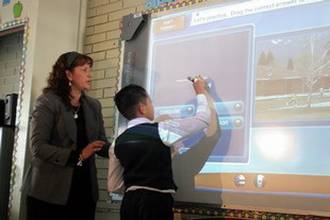
\includegraphics[width=0.5\textwidth]{img/pizzarra.png}  
\small
\caption{Kid interacting with an Electronic Whiteboard}
\label{fig:witheboard}    
\end{figure*} 

\section{Intelligent Tutoring Sistems}
ITS research is the only one of the IT's in general which has as its scientific objective create forms of psychological and social educational knowledge. In some ILEs to motivate the learner, he is placed in realistic contexts and authentic representations of tasks in the real world. Resources are given to the user which will help him do these tasks. The resources in the LE are represented in 2 ways, the first is physically (books, printed images, toys etc.), the other is digitally where devices are used to display images, texts, videos, audios helping to contextualize the activity or the environment itself. Currently there are other devices besides computers that can be used in the LE as Smartphone's, Tablet's, projector's, video game consoles etc. The challenge for LE (as we mentioned before) is to select appropriate resources but must also be a learning sequence that satisfies the user needs and make sense of what is being learned. There are many techniques for establishing learning sequences as \cite{DBLP:conf/um/2003},[14] and [16]. In this case we focus on the simple sequence \cite{ims2012} which has the task of generating a sequence of activities of the subject to be learned by the user. In each of these activities there are precondition rules \cite{ims2012} which serve to make decisions about what to do with activities like hide, show, skip or repeat the activity. The rules require certain values to make these decisions for example when there is an activity that displays information that the user may already know and do not need to see it this activity is skipped or if an activity requires the user to have some age to view it. Fuzzy logic has been previously used in learning environments work as \cite{884142},\cite{DBLP:conf/ifsa/2007-2} the advantage offered by fuzzy logic is that it can work with linguistic variables which take values such as "you are young" and turn it into something measurable as 18 years. We propose to use fuzzy logic on the precondition rules. 
\chapter{Art State} \label{artstate} 
In this section the state of the art in intelligent learning environments, e-learning and context are presented. The learning environments have been 
(Falta aqui)

\section{E-learnign}
Aprendizaje colaborativo basado en recursos adaptativos.

This work consists of an Adaptive Hypermedia System \cite{Valdez2007}, this work is focused on semi-automatic sequencing of educational resources. It builds on information that can be subjective; for example, the user's knowledge, learning style, their predilections and even evaluation; they are perceived differently depending on the context. Sequenced personalized teaching materials; using fuzzy rules and attributes to treat subjective information, involved in the learning process. I n a hypermedia system, such as the Web (W3C, 2008), users surf by  a network of resources for information or to perform some task. In the case of a student, navigation can be part of a complex learning activity; an activity may consist of: search some information, discuss the findings with other students (online), and then make a presentation where resources of different formats and sources are integrated.
In this paper propose: the architecture for a learning environment based on reusable resources, using techniques such as Adaptive Hypermedia and engine adaptation an extension to Simple Sequencing specification where a particular system of fuzzy inference. In include the use of systems fuzzy inference can facilitate the damnation of rules by the instructors, because in the learning process involved usually fuzzy variables.

\section{Learning Environments}
\section{Context}
PCULS
“Personalized context-aware ubiquitous learning system for supporting effective English vocabulary learning” [Chen 2010]. This work consists of a system that supports students in English using a situational approach to learning based on the location of the learner. Detected by wireless positioning techniques, learning time, individual skills of students in English and free time, which enables students to fit your learning content to effectively support the learning of English in a school environment generating vocabulary appropriate to the situation and presenting textual information via mobile phones. When only text information shown this lack of context that was trying to capture in the vocabulary.
 

Procedure system operations:
In Step 1: The learner enters the system through the user interface where the system checks the user's account and free time available to the user.
In Step 2: After the apprentice enters the system, the student agent location automatically determines its location using a location technique based on neural networks.
In step 3 and 4: Based on the location of the learner, the context analyzer agent receives contextual information database user and context. Therefore appropriate agent finder English vocabulary seeks the context of the learner according to the analytical results of context analysis agent fits.
In step 5: Content delivery agent organizes the English learning materials discovered by the search agent material learning English as appropriate content and transmits it to the device of the learner.
In step 6: The message delivery agent transmits the learning content to the learner PDA as a web page or in the form of short message to the cell apprentice. then the trainee returns to step 2 to start the next learning cycle or exit the system, completed the learning process.
The application was tested with two sets of users. they applied a test for each user group with these results.
 
	
Display-based services through identification: An approach in a conference context.
This work combines ubiquitous computing, context, information display and [Hervas 2006] devices, to provide services to the user implicitly, with little or no user intervention feeding context information provided by sensors embedded in devices the environment. Its primary objective is to obtain service information display adaptable to changes in context, providing the same information. They base their research on the identification of users, knowing their profile, their situation in a given underlying information and much other time. Which results in a system that identifies users through RFID cards, and after analyzing generated user information service based on the information display. The whole operation of the service information display is divided into three distinct modules: Context Analysis, generation module mosaics and Composer module. The contextual model represented by an ontology proposed by the authors. The following figure shows the outline of the project is shown.
 
Every moment is available context information filtered according to the ontology and obtained from the system database and embedded sensors in the context (in principle RFID antennas and RFID tags information). The context analysis module is responsible for deciding when a change in the context must lead to changes in display devices. It is also responsible for the system database maintains the consistency of information on these changes. mosaics are generated after an analysis of the background information so that the appropriate and optimal environmental conditions to display information. The generator module provides an XML description of the Mosaic module compounder. From the description of the specific information to be displayed and the mosaic is generated is obtained, publishing through the devices of the environment and taking into account their differences.

 

\chapter{Theory and Background} \label{theoryandbg} 
This chapter overviews the background and main definitions and basic concepts, useful to the development of this investigation work.
\section{Learning environment}

	Learning environment refers to the diverse physical locations, contexts, and cultures in which students learn. Since students may learn in a wide variety of settings, such as outside-of-school locations and outdoor environments, the term is often used as a more accurate or preferred alternative to classroom, which has more limited and traditional connotations�a room with rows of desks and a chalkboard, for example.
The term also encompasses the culture of a school or class�its presiding ethos and characteristics, including how individuals interact with and treat one another�as well as the ways in which teachers may organize an educational setting to facilitate learning�e.g., by conducting classes in relevant natural ecosystems, grouping desks in specific ways, decorating the walls with learning materials, or utilizing audio, visual, and digital technologies. And because the qualities and characteristics of a learning environment are determined by a wide variety of factors, school policies, governance structures, and other features may also be considered elements of a �learning environment.�
Educators may also argue that learning environments have both a direct and indirect influence on student learning, including their engagement in what is being taught, their motivation to learn, and their sense of well-being, belonging, and personal safety. For example, learning environments filled with sunlight and stimulating educational materials would likely be considered more conducive to learning than drab spaces without windows or decoration, as would schools with fewer incidences of misbehavior, disorder, bullying, and illegal activity. How adults interact with students and how students interact with one another may also be considered aspects of a learning environment, and phrases such as �positive learning environment� or �negative learning environment� are commonly used in reference to the social and emotional dimensions of a school or class.

\section{Interactive learning environment}

	Interactive learning is a pedagogical approach that incorporates social networking and urban computing into course design and delivery. Interactive Learning has evolved out of the hyper-growth in the use of digital technology and virtual communication, particularly by students. The use of interactive technology in learning for these students is as natural as using a pencil and paper were to past generations. The Net Generation or Generation Y is the first generation to grow up in constant contact with digital media. Also known as digital natives, their techno-social, community bonds to their naturalized use of technology in every aspect of learning, to their ability to learn in new ways outside the classroom, this generation of students is pushing the boundaries of education. The use of digital media in education has led to an increase in the use of and reliance on interactive learning, which in turn has led to a revolution in the fundamental process of education.
Increasingly, students and teachers rely on each other to access sources of knowledge and share their information, expanding the general scope of the educational process to include not just instruction, but the expansion of knowledge. The role change from keeper of knowledge to facilitator of learning presents a challenge and an opportunity for educators to dramatically change the way their students learn. The boundaries between teacher and student have less meaning with interactive learning.
\section{Intelligent Tutoring System}

An intelligent tutoring system (ITS) is a computer system that aims to provide immediate and customized instruction or feedback to its learners during a task,[joseph p]without intervention from humans. ITSs have maintained the common goal of enabling learners to acquire information in a meaningful and effective manner by employing tools from a range of different technologies to direct the task at hand. There are numerous examples of ITSs being used in both education and professional settings since the mid-1920s. As a result, there is a strong relationship between ITSs, cognitive learning theories and instructional design. As with any mechanism for learning, ITSs have experienced its share of successes and limitations with continuous research investigating the best approach to addressing the dialogues and affective responses to learning.
Research in ITS organizes the "problem" in [1] knowledge about a domain, [2] knowledge about the learner, and [3] pedagogy (knowledge of teaching strategies). The major components of a typical ITS are an expert (or domain) model, student model and tutoring model. The expert model should be able to solve the problems the tutoring module submits to the students. The tutor module controls the interaction with the student, based on its teaching knowledge and comparisons between the student model and the domain knowledge. The student model reflects what the machine can infer about the student's cognitive state
\section{Intelligent learning environment}

An intelligent learning environment is a new kind of intelligent educational system, which combines the features of traditional Intelligent Tutoring Systems (ITS) and learning environments. An intelligent learning environment (ILE) includes special component to support student-driven learning, the environment module. The term environment is used to refer to that part of the system specifying or supporting the activities that the student does and the methods available to the student to do those activities [8]. Some recent ITS and ILE include also a special component called manual which provides an access to structured instructional material. The student can work with the manual via help requests or via special browsing tools exploring the instructional material on her own. An integrated ILE, which includes the environment and the manual components in addition to regular tutoring component, can support learning both procedural and declarative knowledge and provide both system-controlled and student-driven styles of learning.
\section{Fuzzy Logic}

	Zadeh introduced the term fuzzy logic in his work �fuzzy sets�, where he described the mathematics of the fuzzy set theory in 1965.
	Fuzzy logic gives the opportunity to model conditions that are defined with imprecision.
	The tolerance of the fuzzy in the process of human rezoning suggests that most of the logic behind the human rezoning is not the traditional bi-valued logic, or even the multi-valued, but the logic with fuzzy values, with fuzzy connections and fuzzy rules or inferences.

\subsection{Fuzzy sets}

	Fuzzy sets are an extension of the classic set theory and, as it name implies it, it is a set with boundaries not well defined, this means that the transition of belonging or not belonging to certain set is gradual, and this smooth transition is characterized by grades of membership that gives the fuzzy sets flexibility in modeling linguistic expressions commonly used, such as �the weather is cold� or �Gustavo is tall�.
 
Figure 2.1.Key-Value example.

\subsection{Fuzzy logic controller}

	Fuzzy control is a control method based on fuzzy logic. Just as fuzzy logic can be described simply as �computing with words rather than numbers� fuzzy control can be described simply as �control with sentences rather than equations�.
	The collection of rules is called a rule base. The rules are in the familiar if-then format, and formally the �if� side is called the antecedent and the �then� side is called the consequent.
	Fuzzy controllers are being used in various control schemes; the most used is the direct control, where the fuzzy controller is in the forward path in a feedback control system. The process output is compares with a reference, and if there is a deviation, the controller takes action according to the control strategy.
	In a feed forward control a measurable disturbance is being compensated, it requires a good model, but if a mathematical model is difficult or expensive to obtain, a fuzzy model may be useful. Fuzzy rules are also used to correct tuning parameters. If a nonlinear plant changes operating point it may be possible to change the parameters of the controller according to each operating point. His is called gain scheduling since it was originally used to change process gains. 
	A gain scheduling controller contains a linear controller whose parameters are changed as a function of the operating point in a preprogrammed way. It requires thorough knowledge of the plant, but it is often a good way to compensate for nonlinearities and parameter variations. Sensor measurements are used as scheduling variables that govern the change of the controller parameters, often by means of a table look-up.
\section{Learning object}


Learning object design raises issues of portability, and of the object's relation to a broader learning management system.
Learning objects are the basic elements of current Learning Management Systems (LMS) and are the focus of standardization initiatives whose goal is defining open technical standards and their characteristic metadata [6]. The most important initiatives are the Advanced Distributed Learning Initiative (ADL-SCORM) [7], the Instructional Management System Project (IMS) [8], the Alliance of Remote Instructional Authoring Distribution Networks of Europe (ARIADNE) [9], and the IEEE Learning Technology Standards Committee [10]. The main objective of these open standards is to enable the interoperability of learning objects between different LMSs and Learning Objects Repositories (LORS). Basic metadata schema specifications for learning objects include: Learning Object Metadata (LOM). Based on the Dublin Core metadata [11] this specification defines a set of meta- data elements that can be used to describe learning resources. LOM Includes educational, relation, technical, and classification elements [7]. Content Aggregation Model (CAM). CAM defines a package for the aggregation, distribution, management, and deployment of learning objects. Defines an organization element which contains information about one particular, passive organization of the material, the organization for now is limited to a tree structure [8]. Learner Information (LI). A collection of information about a learner or a producer of learning content, the elements are based upon accessibilities; activities; affiliations; competencies; goals; identifications; interests; qualifications, certifications and licenses; relationship; security keys; and transcripts [8]. Sequence and Navigation (SN). SN defines a method for representing the intended behavior of an authored learning experience such that any Learning Technology system (LTS) can sequence discrete learning activities in a consistent way. Provides a rule based sequencing of behaviors [7]. These standards have been the basis for various research projects in eLearning [11] and also extensions to support adaptability have been proposed [13], [14], [15]. Certain limitations of these specification initiatives have been noticed mainly regarding their weak support for the instructional design of the educational resources and pedagogy [16]. 

\section{NoSQL}

In computing, NoSQL (sometimes called "not only SQL") is a broad class of systems management databases that differ from the classical model of relational database management system (RDBMS) in important aspects, the most prominent is that they are not using SQL as the primary query language. The stored data do not require fixed structures such as tables, typically do not support JOIN operations, not fully guarantee ACID (atomicity, consistency, isolation and durability), and usually scale well horizontally. The NoSQL systems are sometimes called "not only SQL" to underline the fact that they can also support query languages like SQL. The NoSQL databases Systems grew with major Internet companies like Google, Amazon, Twitter and Facebook. These had to face challenges with data processing than traditional RDBMS not solved. With the growth of the web in real time there was a need to provide processed information from large volumes of data that had more or less similar horizontal structures. These companies realized that the performance and real-time properties were more important than consistency, in which the traditional relational data bases devoted a lot of processing time. 
In that sense, often, NoSQL databases are highly optimized for operations retrieve and add, and usually do not offer much more than the functionality of store records (eg key-value storage) that we can see on figure \ref{keyvalue}. The loss of flexibility at run time compared to conventional systems SQL, is offset by significant gains in scalability and performance when it comes to certain data models.

 \begin{figure}[ht!]  
\centering  
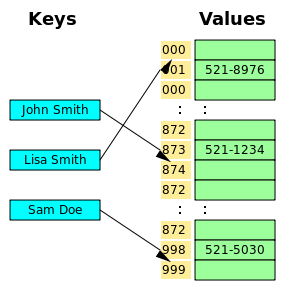
\includegraphics[scale=1]{nosqlejemplo}
\quad  
\caption{Key-Value Storage}  
\label{keyvalue}  
\end{figure}

\subsection{Key-Value example}

Typically the modern relational data bases have shown little efficiency in certain applications that use data intensively, including indexing of a large number of documents, presentation pages sites with high traffic, and sites audiovisual streaming. Typical implementations of RDBMS have tuned either for a small but frequent reads and writes or a large set of transactions that have few write accesses amount. On the other hand it can serve NoSQL lot of load of reads and writes.
\subsection{Advantages of NoSQL systems}

This way of storing information provides certain advantages over relational models. Between the most significant advantages can include:
They are executed in machines with limited resources: These systems, unlike based systems SQL, not just require computer, so they can be mounted on machines of a lower cost.
Horizontal Scalability: To improve the performance of these systems is achieved simply adding more nodes, with the only operation of the system indicate which nodes are available.
Can handle large amounts of data: This is because it uses a distributed structure, Hash many cases using tables.
Do not generate bottlenecks: The main problem with SQL systems is that they need to transcribe each sentence to be executed, and each complex sentence also requires a level even more complex implementation, which is an entry point in common, that before many requests can slow down the system.

\subsection{Main differences with SQL databases}

Some of the most remarkable differences we can find between NoSQL systems and SQL systems are:
Do not use SQL as a query language. Most NoSQL databases avoid using this kind of language or use it as a language support. To give some examples, Cassandra uses CQL language, MongoDB uses JSON or BigTable uses GQL.
Not use fixed structures as tables for storing data. Let you use other types of storage models as key-value systems, objects or graphs.
Tend not allow JOIN operations. By having a data volume so extremely large is often desirable to avoid the JOIN. This is because, when the operation is not the search for a key, the overhead can become very costly. The most straightforward solutions consist of denormalising data or perform the JOIN by software in the layer application.
Distributed architecture. The relational databases are typically centralized in a single machine or in a master-slave structure, however in cases NoSQL information it can be shared across multiple machines through mechanisms of distributed hash tables.

\subsection{Types of NoSQL databases}

Depending on how you store the information, we can find various types other than NoSQL databases. Consider the most commonly used types.
Key-Value Database: They are the base model popular NoSQL data, besides being the simplest in terms of functionality. In this type of system, each element is identified by a unique key, allowing the retrieval of information very quickly, which is usually stored information as a binary large object (BLOB). They are characterized by being very efficient for both readings and for scriptures. Examples of this type are Cassandra, HBase or BigTable.
 


Document databases: They are the base model popular NoSQL data, besides being the simplest in terms of functionality. In this type of system, each element is identified by a unique key, allowing the retrieval of information very quickly, which is usually stored information as a binary large object (BLOB). They are characterized by being very efficient for both readings and for scriptures we can see an example of this kind of data base on the figure 2.3. Examples of this type are Cassandra, HBase or BigTable. 
\begin{figure}[ht!]  
\centering  
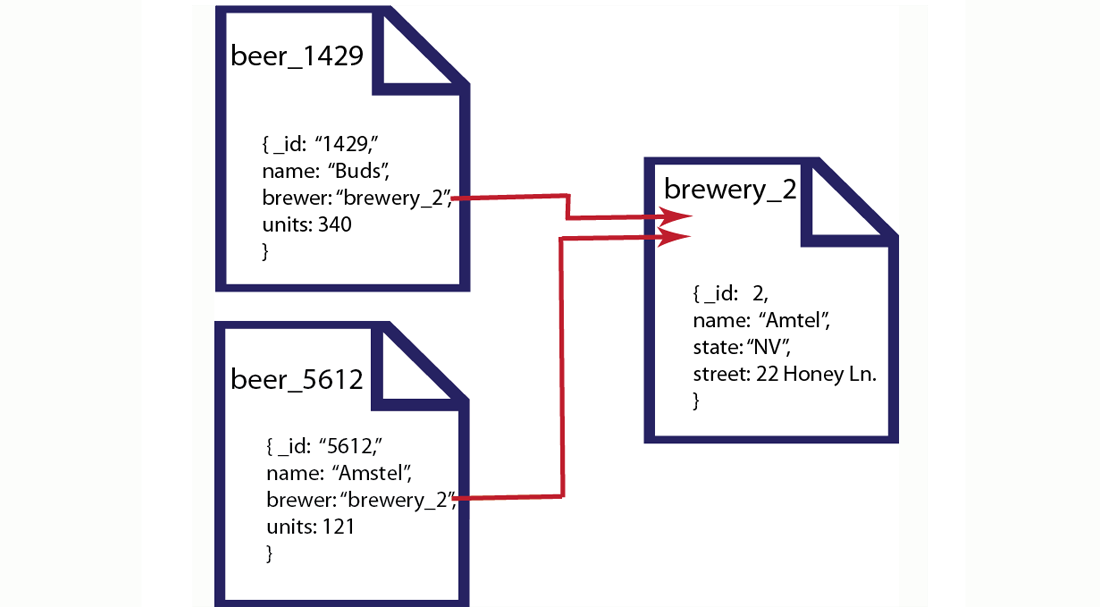
\includegraphics[scale=1]{basededatosdoc}
\quad  
\caption{Document Database Example}  
\label{bddd}  
\end{figure}

Graph databases: In this type of databases, information is represented as nodes of a graph and its relations with the edges thereof (Figure 2.4), so that you can make use of graph theory to cover it. To remove the most of this type of database, its structure must be fully normalized, of so that each table has a single column and each relationship both. This type of database provides a more efficient navigation between relationships vs a relational model. Examples of this type are Neo4j, InfoGrid or Virtuoso.

\begin{figure}[ht!]  
\centering  
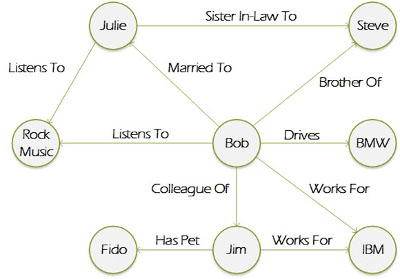
\includegraphics[scale=0.75]{Graph-database}
\quad  
\caption{Graph Database Example}  
\label{bdg}  
\end{figure}

\subsection{Examples of NoSQL databases}

Here are some examples of the most commonly used nosql databases.

Cassandra: This is a database created by Apache key-value type. It has its own language for CQL (Cassandra Query Language) queries. Cassandra is a Java application so it can run on any platform that has the Java Virtual Machine.
 
\begin{figure}[ht!]  
\centering  
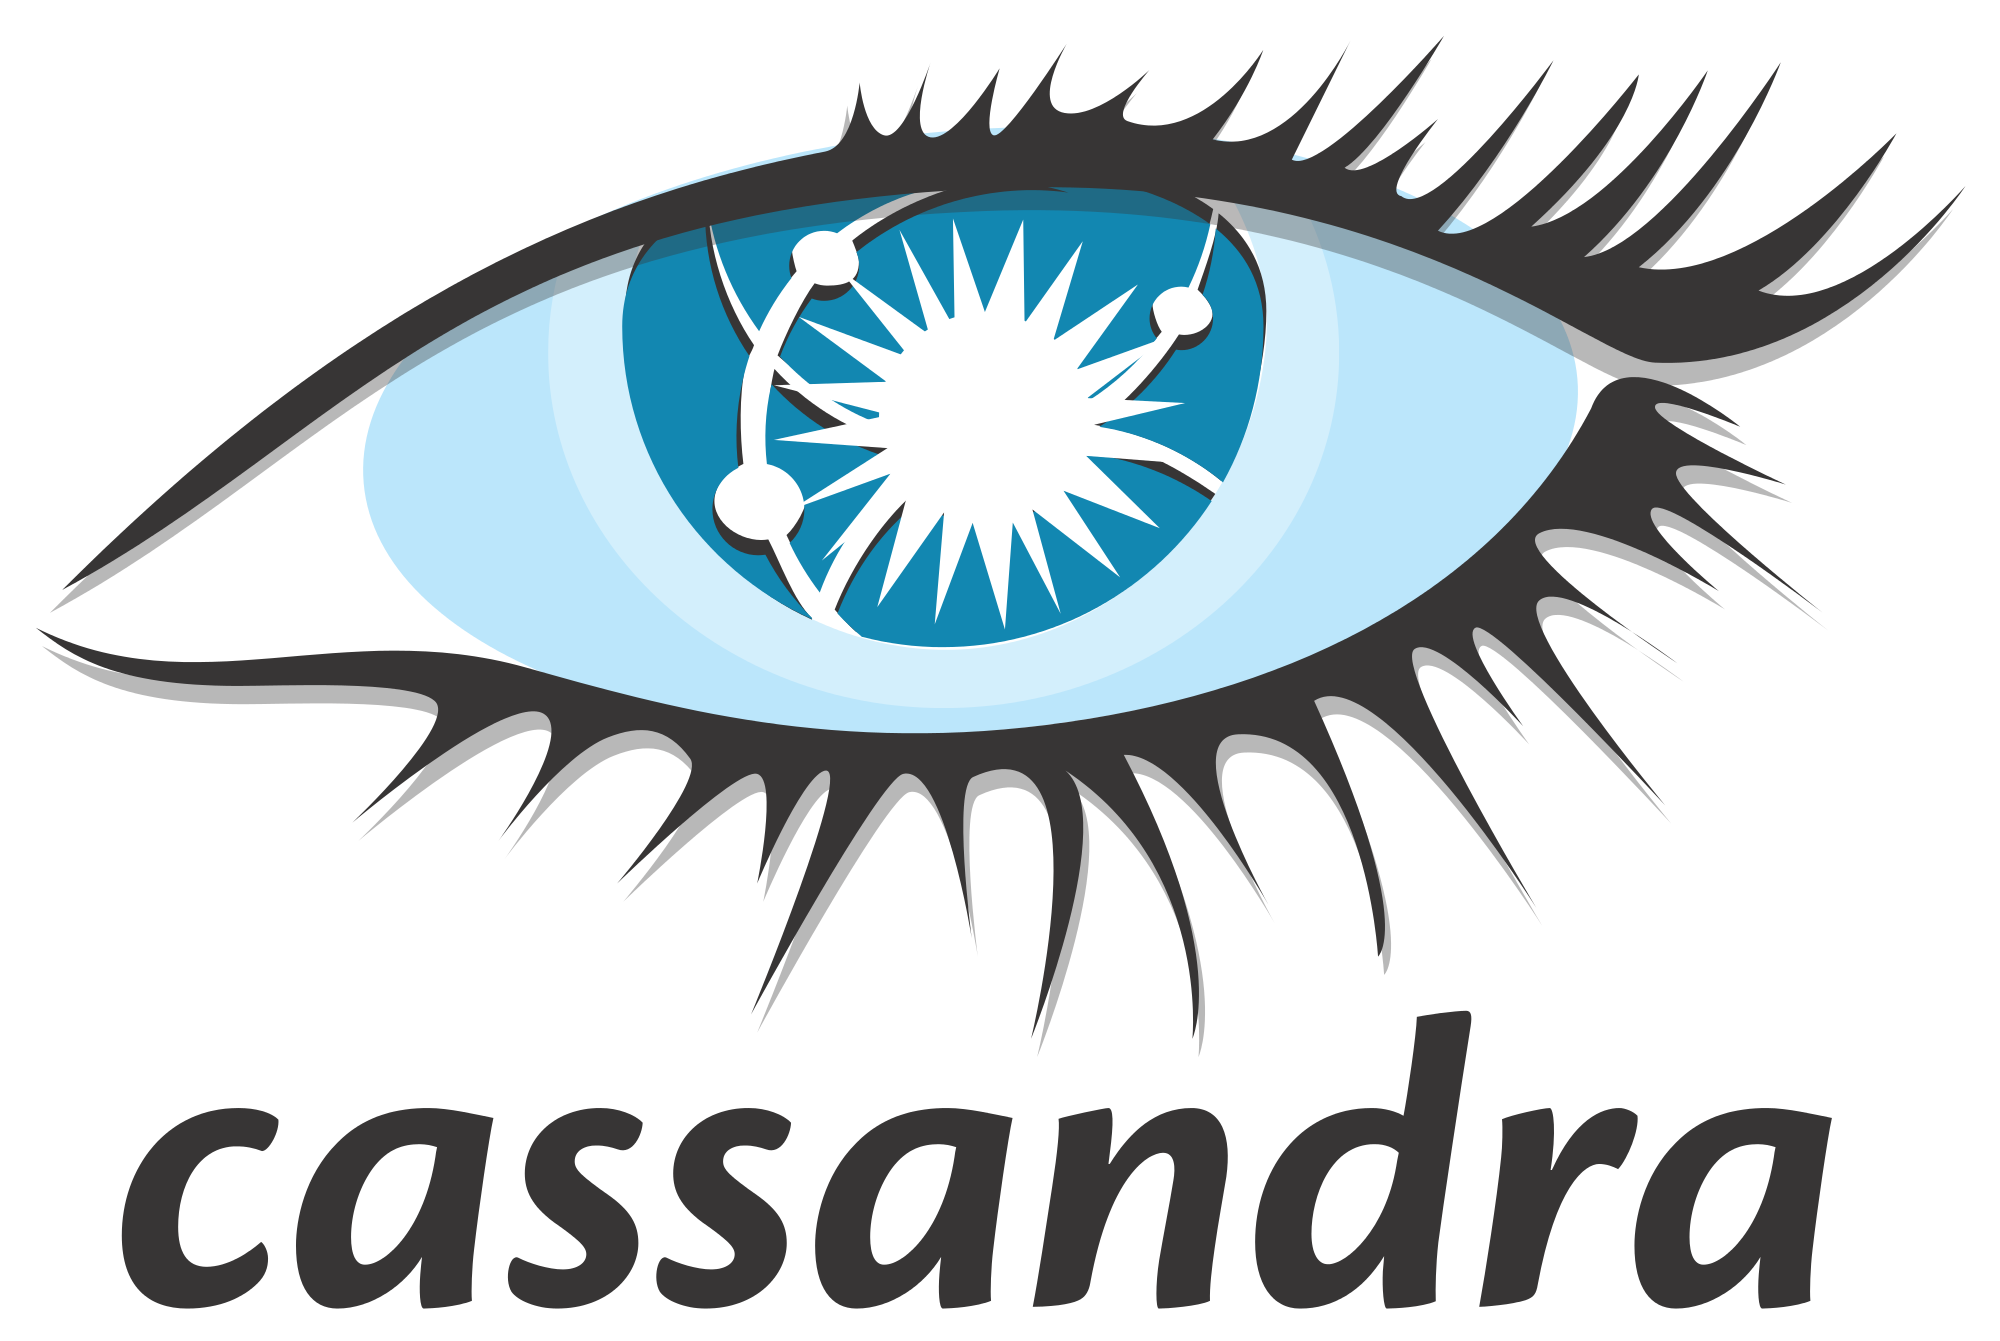
\includegraphics[scale=0.1]{cassandra}
\quad  
\caption{Nosql Database Cassandra}  
\label{bdg}  
\end{figure}


MongoDB: This is a database created by 10gen document-oriented type, Free scheme is meaning that each input can have a different data schema that has nothing to do with the rest stored records. It's pretty quick to run its operations as it is written in C ++ language. For information storage, uses a proprietary system known document with the BSON name, which is an evolution of the popular JSON but with the peculiarity that can store binary data. Soon, MongoDB has become one of the bases of popular NoSQL data by developers.
 
\begin{figure}[ht!]  
\centering  

\includegraphics[scale=1]{mongo}
\quad  
\caption{Nosql Database MongoDB}  
\label{bdg}  
\end{figure}


CouchDB: It is a system created by Apache and written in Erlang language that works in most POSIX systems, including GNU / Linux and OSX, but not in Windows systems. The most important features include the use of Restfull HTTP API as an interface and JavaScript as the main language of interaction. For storage of data files used JSON.Allows creation of views, which are the mechanism that allows the combination of documents return values of several documents, ie, CouchDB allows performing operations JOIN Typical SQL.

\begin{figure}[ht!]  
\centering  

\includegraphics[scale=1]{couchdb}
\quad  
\caption{Nosql Database CouchDB}  
\label{bdg}  
\end{figure}


\chapter{The Proposed Method} \label{proposmeth} 
In this chapter, an architecture for developing interactive learning environments is proposed. The architecture allows the use of techniques of adaptive hypermedia systems and use in interactive environments. This architecture has as resources environmental learning objects, which are presented to users through the various devices that can be part of this environment and are organized by a sequence based on Simple Sequencing. Also a new method to automate the measurement of the level of attention of the user without using invasive methods. In Figure X we can observe the components of this architecture. As this environment has multiple configurations of use, sometimes it can help a fuzzy inference system to adapt the information presented by the environment to users. The components of the architecture are described in detail.

\section{Environment}
Los ambientes inteligentes son espacios con sistemas embebidos, sensores y tecnolog�as de informaci�n y comunicaci�n que se van haciendo imperceptibles para el usuario a media que van siendo integrados en objetos f�sicos, infraestructuras, el entorno en que vivimos, el trabajo y muchos otros ambientes. Los ambientes inteligentes interactivos facilitan herramientas con las cuales los usuarios pueden interactuar, lo que hace que este espacio sea interactivo por lo que la computaci�n se aproxima m�s al usuario. Existen otros tipos de ambientes como e-learning que son ambientes de aprendizaje virtuales donde un usuario aprende individualmente ciertos temas a partir de objetos de aprendizaje. Los trabajos en este tipo de ambientes de aprendizaje han utilizado diferentes t�cnicas para secuenciar y seleccionar los objetos de aprendizaje para cubrir las necesidades de aprendizaje del individuo como el secuenciado simple (referencia a la tesis del profe). 

Actualmente existen ciertas limitaciones con los ambientes inteligentes por ejemplo:
\begin{itemize}	
\item Los ambientes de aprendizaje est�n pensados para que los objetos de aprendizaje sean utilizados por un usuario a la vez.
\item La informaci�n contextual aveces no es considerada.
\item Normalmente el ambiente no puede ser llevado a otros lugares sin tener que hacerle modificaciones.
\item Algunos trabajos con ambientes utilizan dispositivos que no son tan avanzados como lo son ahora a dem�s de que se han hecho mas accesibles econ�micamente.

Proponemos generar un ambiente que gracias a un servicio web sea capaz de atacar todas las limitaciones que observamos en los ambientes de aprendizaje actuales. gracias a los servicios web podemos crear repositorios que pueden estar disponibles siempre y cuando exista una conexion a internet, pero que pasa con aquellos lugares donde no exista tal conexion, 




\section{ELO}
A standard learning object is defined in [2]. The teacher prepares teaching materials using content from various sources; select different pieces of information that subsequently assembled to form the course or class to teach. Learning objects are based on this methodology, seeing the didactic content as a component that is designed to combine with others and to be used in different contexts; learning objects usually have the following characteristics: 
�	They are self-contained. Each learning object can be used independently. 
�	Are reusable. A learning object can be used in different contexts, for multiple purposes. 
�	Can be added. Learning objects can be grouped into collections, after being presented with a traditional course structure. 
�	Are labeled with metadata. Each learning object has associated certain in-formation that describes it. This facilitates reuse by automatic means.
We propose a learning environment that uses a new type of learning object which we call "environmental learning object" (ELO) these objects include additional metadata that can be used to identify and manage content for their use in ubiquitous devices: we considered input and output devices e.g. interactive tables, wall projections, monitors, tablets, cameras, microphones and speakers.
By tagging through the metadata we can make a selection of learning objects to create and manage different contexts when applied to a learning environment as we can note in Figure.
Where each learning object is selected and routed to a device that operates its utility like a sound file that can�t be used on a monitor maybe on a Smartphone or a tablet pc, these are the types of problems that can occur when using these learning objects. Also this ELO will give contextual information for feedback. Then the learning object is attached to the sequence as we can see on the figure 3.1.
\section{Fuzzy simple sequencing}
Simple sequencing standard[18] [19], which allows sequencing of this type of learning objects. First an activity tree with n number of activities is determined by the teacher, selecting the learning objects to be used per activity and adding fuzzy pre-condition rules that consider the context and user model to determine the sequence, for example:
IF Context.Temperature is HIGH and Session.Activity.Place is OUTSIDE
THEN
this.Precondition. = SKIP.
Then context information is obtained from users using the sensors mentioned above, each activity will have 1 or more environmental learning objects, thanks to the metadata included in the learning objects will be displayed in the appropriate device for example if we have a web page can be displayed on a monitor, a questionnaire on a tablet, a video projected on a wall, sound on speakers, an interactive game on the table as we can see in Figure 3.
The main components of the Simple Sequencing standard are the Learning Activities and the Activity Tree. A Learning Activity is defined as a pedagogically neutral unit of instruction, knowledge, evaluation, etc. Learning Activities can have nested sub-activities arbitrary depth. 
There is an implicit hierarchy of containers in the tree. Depending on the application concept labels can be applied to learning activities. Only leaf nodes can be associated with Resources Activity (the equivalent of Learning Objects).An example of the configuration obtained by sequencing can be observed in Figure 3.2. The tree is traversed as follows from the root there is the General activity (can be any subject in particular) with 2 nodes in it, we see that has the attribute "forwardOnly" on true, this means they have to be traveled sequentially by users, the first activity is a pre-evaluation, which is associated with a learning object in this case a test that contains a rule that makes the activity is carried out or otherwise will not advance to the next activity, as specified in the Pre\_condition rule.
When a learning sequence is generated learning activities are established and they not change, what changes is the action as if you skip, performed, jump, hide, repeat or show an activity, this decision is taken by the rules of precondition. In this paper we seek to generate diversity of resources displayed in the activities adapting the resources of the activity to the user,  for example we have an introductory activity of a particular subject and 2 users of different ages perform the activity, the first user of 25 years will be shown more detailed and textual information, while the second user of 6 years of age is in a very early stage of learning resources that show you are easier to understand and have more audio-visual con-tent. With fuzzy logic generate inputs for use in the precondition rules for example: fuzzy rule if user.age is low and user.academic\_level is low then user.level is begginer. On the precondition rule we will use the output of the fuzzy rule will use the output of that fuzzy rule as follows if user=begginer then pre\_condition = show. Thus a set of resources is obtained for a novice user and these are shown on the right devices for each resource through a web browser running in this device as we can see on the figure 1.
Los recursos son los objetos de aprendizaje, los cuales como ya sabemos pueden ser cualquier video, imagen, audio o texto, para esta investigaci�n utilizamos una gran cantidad de im�genes videos y audios. Con un aproximado de 100 im�genes, 10 videos y m�s de 20 audios fue lo que formo parte de cada una de las configuraciones del ambiente. Al inicio las dimensiones de las im�genes fueron un problema ya que no todos los dispositivos ten�an resoluciones similares, tiempo despu�s se implemento una forma de ajustar las im�genes a la resoluci�n de cada pantalla o proyector. Al igual que las im�genes los videos tuvieron el mismo problema ya solucionado en las �ltimas versiones.
\section{Devices}
\section{Master / User}
\chapter{Case of Study} \label{expres} 
\section{Experiments}
In this chapter we present the relevant experiments that were done to test the proposed method. Subsequently, it shows the implementation of the method in a adaptive learning environment used as case of study, deployed in different places. A wide explanation of the system interfaces and its functionality is explained also.

In this particular experimental scenario, we propose some guidelines and follows some guidelines from related work like the work of Hervas\cite{bravo2005display}, Chen\cite{Chen2007}, Garcia-Valdez\cite{mariotesis}, and they are briefly explained next.
\begin{itemize}	

\item • Hypothesis: before running the experiment we must form an hypothesis. It is important to be concise and restrictive about this hypothesis, and design an experiment that tests the hypothesis. For example, an hypothesis can be that adaptive environment A adapts and presents better learning objects to the user and the user likes and learn more than the environment B. In that case,the experiment should test the acceptance and assimilation of the environment including content, ease of use etc.

\item • Controlling variables: when comparing a few learning environments on a certain hypothesis, it is important that all variables that are not tested will
stay fixed. For example, suppose that we wish to compare the acceptance and assimilation of the environment A and environment B, that both use
different technologies. 

\item • Generalization power: when drawing conclusions from experiments, we may desire that our conclusions generalize beyond the immediate context of the experiments. When choosing an environment for a real application, we may want our conclusions to hold on the deployed system. Generally speaking, the more diverse the data used, the more it can generalize the results.
\end{itemize}

The next sections show a comprehensive description of the experimental setup for experiments, as well as results obtained in the experiments. Each method was tested
using different topics and context. This chapter ends with the description of the functionality of the prototype used to validate the method utilized in the experiments.

\section{Adaptive Learning Environment topic 1}
In earlier implementations of the adaptive environment several experiments were done to test the behavior and the performance. For the experiment the proposed hypothesis is The acceptance and accuracy of the content showed in the adaptive learning environment. The first experiment presents and adaptive learning environment used to teach the topic "El himno nacional Mexicano". llevado a cabo en las instalaciones del instituto tecnologico de tijuana. 
\subsection{Devices}
Los dispositivos usados en este experimento se describen a continuacion. Se necesito de un servidor para manejar las peticiones, almacenar los objetos de aprendizaje, generar la secuencia de aprendizaje y mantener el servicio web activo. En este caso el servidor era una computadora Gateway fx6850 el cual cuenta con 12gb de ram y procesador intel i7 de segunda generacion. se utilizaron 3 monitores de diferentes resoluciones el primero de 1440x900 pixeles, el segundo de 1600x900 y el tercero de 1980x1080 pixeles. Lo que genero un problema a la hora de desplegar imagenes o videos pero se tomaron medidas para adaptar el contenido a diferentes resoluciones. Una tablet nexus7 con la cual el usuario podia controlar la navegacion entre actividades y contestar algunos cuestionarios. y audifonos para el sonido.

\begin{figure}[ht!]  
\centering  
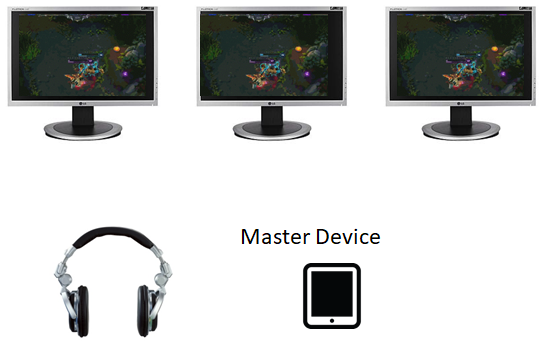
\includegraphics[scale=1]{ambiente2}
\quad  
\caption{Configuration of the first adaptive environment}  
\label{ambiente2}  
\end{figure}
  

\subsection{Topic/Content}
Seleccionamos el tema de el himno nacional mexicano por la razon de que nos parecio un tema de interez general y por lo tanto digerible para diferentes edades y personas.
se comenzo con una breve historia del himno nacional involucrando a sus autores tanto de musica como de letra y una breve sinopsis de cada uno de ellos en la figura \ref{Nuno2} podemos observar una imagen con los 2 personajes pero se muestran 2 imagenes de cada una de los autores, dependiendo del usuario se muestra una u otra imagen.
\begin{figure}[ht!]  
\centering  
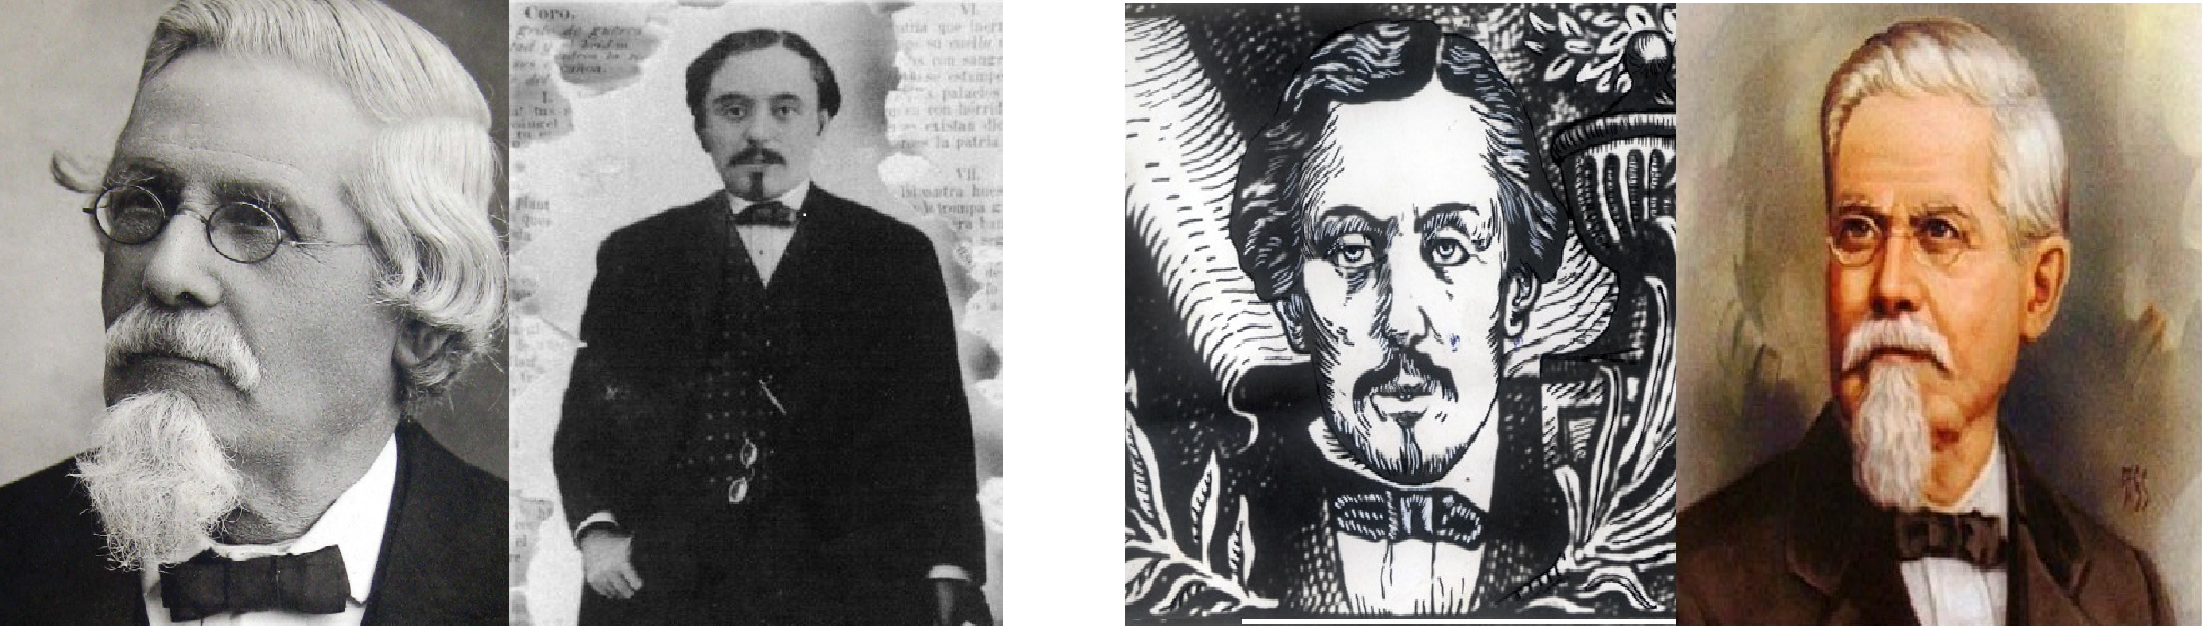
\includegraphics[scale=.25]{Jaime_Nuno2}
\quad  
\caption{2 learning objects.}  
\label{Nuno2}  
\end{figure}

Como lo mencionamos se manejan 3 tipos de usuarios tomando como referencia su edad. basado en el rando de edad un sistema difuso elige que contenido mostrar al usuario. en la imagen anterior \ref{Nuno2} se muestran las imagenes de los autores del himno nacional pero para el tipo de usuario 2 y 3. dependiendo del tipo de usuario cada una de las actividades puede cambiar y hacerce un poco mas digerible, por ejemplo para el usuario 3 que se supone un usuario mas metodico y que tiene en su mayoria tiene mejor aceptacion de informacion compleja se le muestra mas texto, graficas y tablas que quiza son mas dificiles de entender para los usuarios 1 y quiza al usuario 2. entonces es la misma actividad de aprendizaje pero con pequeños cambios con respecto a los diferentes usuarios. 

\subsection{Users}
Los usuarios para este experimento fue una muestra de compañeros de laboratorio, maestros, amigos e hijos de compañeros un grupo de usuarios 10 de diferentes perfiles (tabla 1) con el prototipo del ambiente para ver la impresión que tuvieron realizar una actividad de aprendizaje y obtener retroalimentación de ellos. Este ambiente está planeado para usarse en aéreas grandes pero en este caso se uso un espacio pequeño para la prueba. Para este caso solo se tomaron la edad y el nivel académico el cual va desde 1 hasta 21 donde 1 es primer año de primaria y 21 tiene grado de doctor como lo podemos observar en la tabla \ref{tab:users1}.

\begin{table}
\centering
\small
\captionsetup{font=footnotesize}
\caption{List of users participating in the experiment.}
\label{tab:users1} 

\small
\begin{tabular}{p{3cm} p{3cm} p{3cm} }
\hline{\smallskip}
User & Age	& Academic level\\
\noalign{\smallskip}\hline\noalign{\smallskip}
\small{	1	}& \small{	6	}& \small{	1	}\\
\small{	2	}& \small{	48	}& \small{	19	}\\
\small{	3	}& \small{	23	}& \small{	17	}\\
\small{	4	}& \small{	23	}& \small{	18	}\\
\small{	5	}& \small{	23	}& \small{	18	}\\
\small{	6	}& \small{	24	}& \small{	17	}\\
\small{	7	}& \small{	31	}& \small{	19	}\\
\small{	8	}& \small{	35	}& \small{	20	}\\
\small{	9	}& \small{	45	}& \small{	21	}\\
\small{	10	}& \small{	29	}& \small{	19	}\\
\hline

\end{tabular}
\end{table}

\subsection{Survey}

Cuando los usuarios terminaron de utilizar el ambiente se les realizo una pequeña encuesta, esta encuesta consistía en 5 preguntas sobre su experiencia al utilizar el ambiente preguntas como si se le dificulto utilizarlo o si fue de su agrado los recursos mostrados, con el objetivo de obtener retroalimentación de los usuarios para hacer futuras mejoras y modificaciones que se muestra en la tabla \ref{users2}.
\begin{table}
\small
\centering
\captionsetup{font=footnotesize}
\caption{List of users participating in the experiment.}
\label{tab:users2} 

\small
\begin{tabular}{p{12cm} p{4cm} }
\hline\noalign{\smallskip} 
Question & Answers \\
\noalign{\smallskip}\hline\noalign{\smallskip}\hline
\small{1.From 1-10 how easy it was use the environment? } & \small{1-10[  ]} \\ \hline  
\small{2.From 1-10, how was your satisfaction about the information displayed in the environment? } & \small{1-10[  ]} \\ \hline
\small{3.Did you like the idea of using various visual elements?  } & \small{1. Yes 2.No} \\ \hline 
\small{4.Was necessary technical assistance to use the environment?   } & \small{1. Yes 2.No} \\ \hline   
\small{5.Would you recommend the use of this environment to others?  } & \small{1. Yes 2.No} \\ \hline 
\hline
\noalign{\smallskip}\hline
\end{tabular}
\end{table}

\section{Adaptive Learning Environment topic 2}
For this part of the study users immersed in an exhibitor that gave them visual and aural information as shown in Figure \ref{fig:environment} on a topic selected based on various criteria, such as the location of the study on this occasion was a interactive museum and the festival of children’s day approaching we try to use a simple theme and it will bring awareness so we decided to use the theme of water where information was displayed as the uses of the same, its cycle, forms of energy that could generate, health, and the importance of it for the planet. Each of users are generating an account on the system to register their activity, after that we were made a brief explanation of how it worked the exhibitor others based on observation no longer required this explanation. The user took a tablet that was the how the user interacted with the exhibitor, with which had control of the flow of information, as the information was a sequence at the end of the last activity was a questionnaire on the information received besides a survey.

\begin{figure}[htbp]
\centering
\subfigure[User interacting with the environment.]{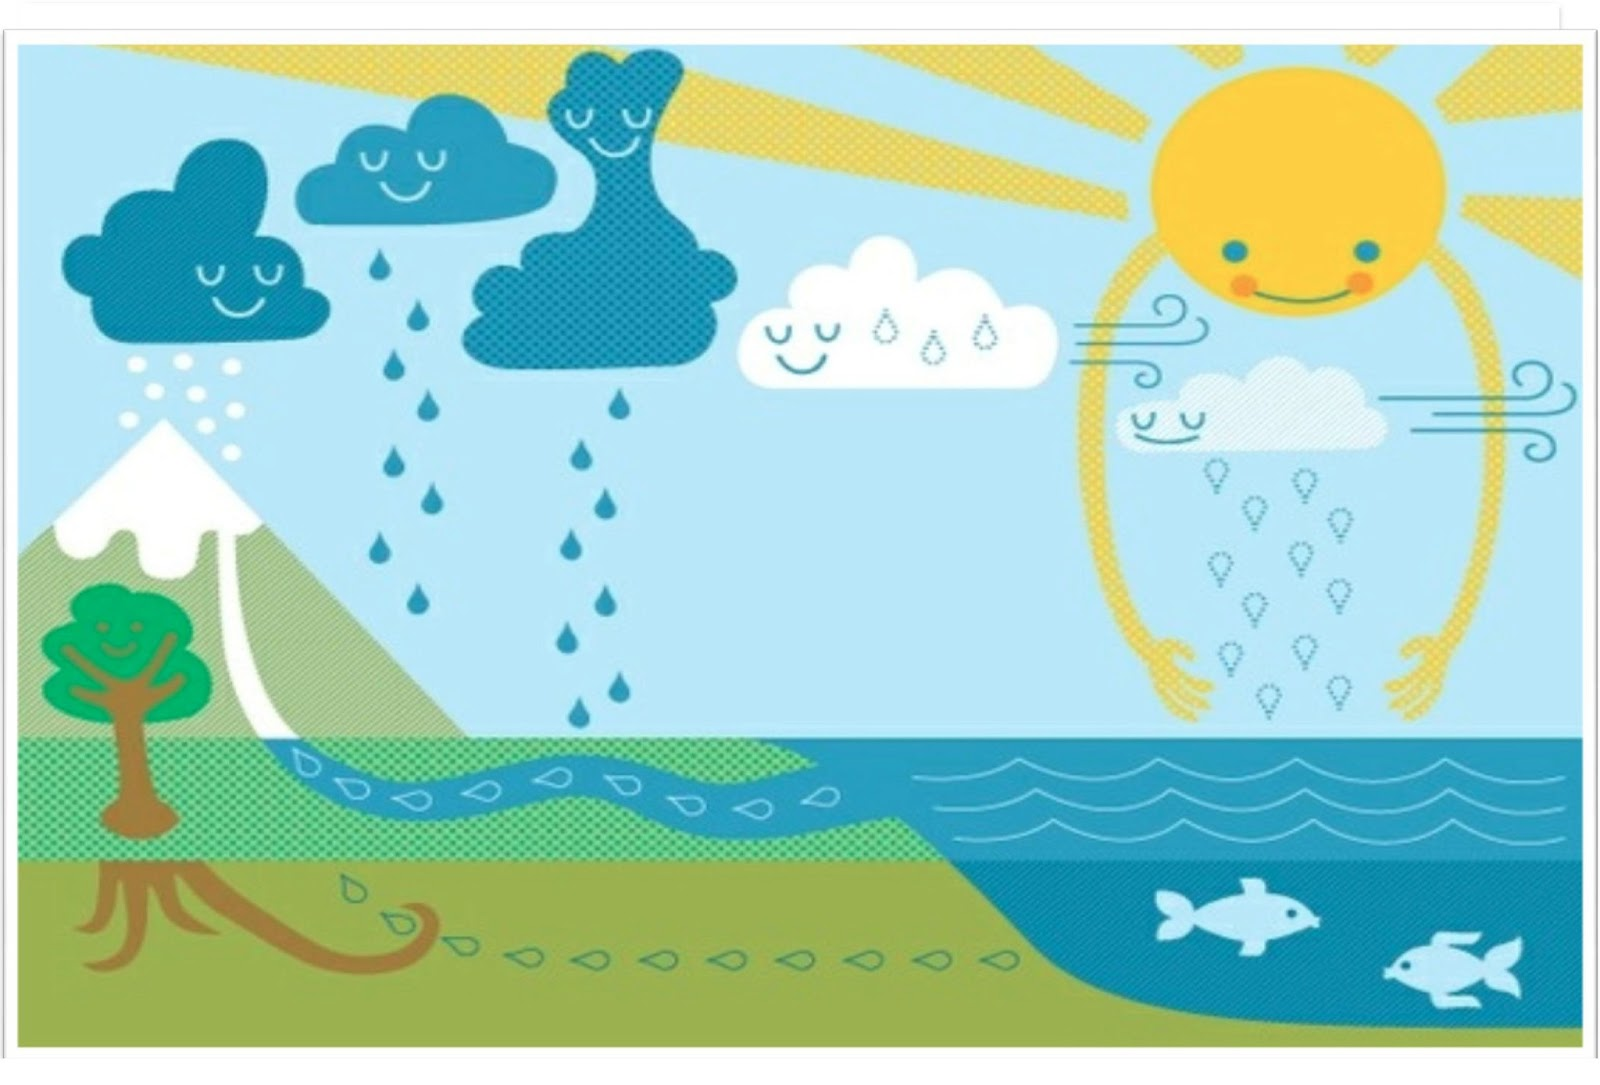
\includegraphics[width=40mm]{agua}}\hspace{10mm}
\subfigure[Front view of the equipt.]{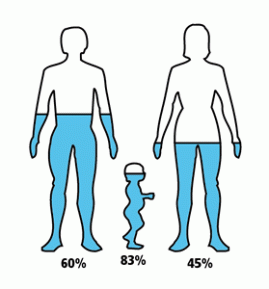
\includegraphics[width=40mm]{agua3}}{10mm}
\caption{The environment.} \label{fig:environment}
\end{figure}

\subsection{Devices}
Los dispositivos usados en este experimento se describen a continuacion. Se necesito de un servidor para manejar las peticiones, almacenar los objetos de aprendizaje, generar la secuencia de aprendizaje y mantener el servicio web activo. En este caso el servidor era una computadora Mac Pro 2014 la cual cuenta con 12gb de ram y procesador intel xeon. se utilizaron 3 proyectores de las mismas resoluciones a diferentes tamaños organizados como se puede observar en la figura \ref{trompo1}. una computadora adicional que realizo diversas tareas como mostrar el contenido de 2 proyectores y reproducir el audio,  una laptop para mostrar contenido en el tercer proyector y una laptop mas donde para obtener los datos del sensor kinect. 

\begin{figure}[ht!]  
\centering  
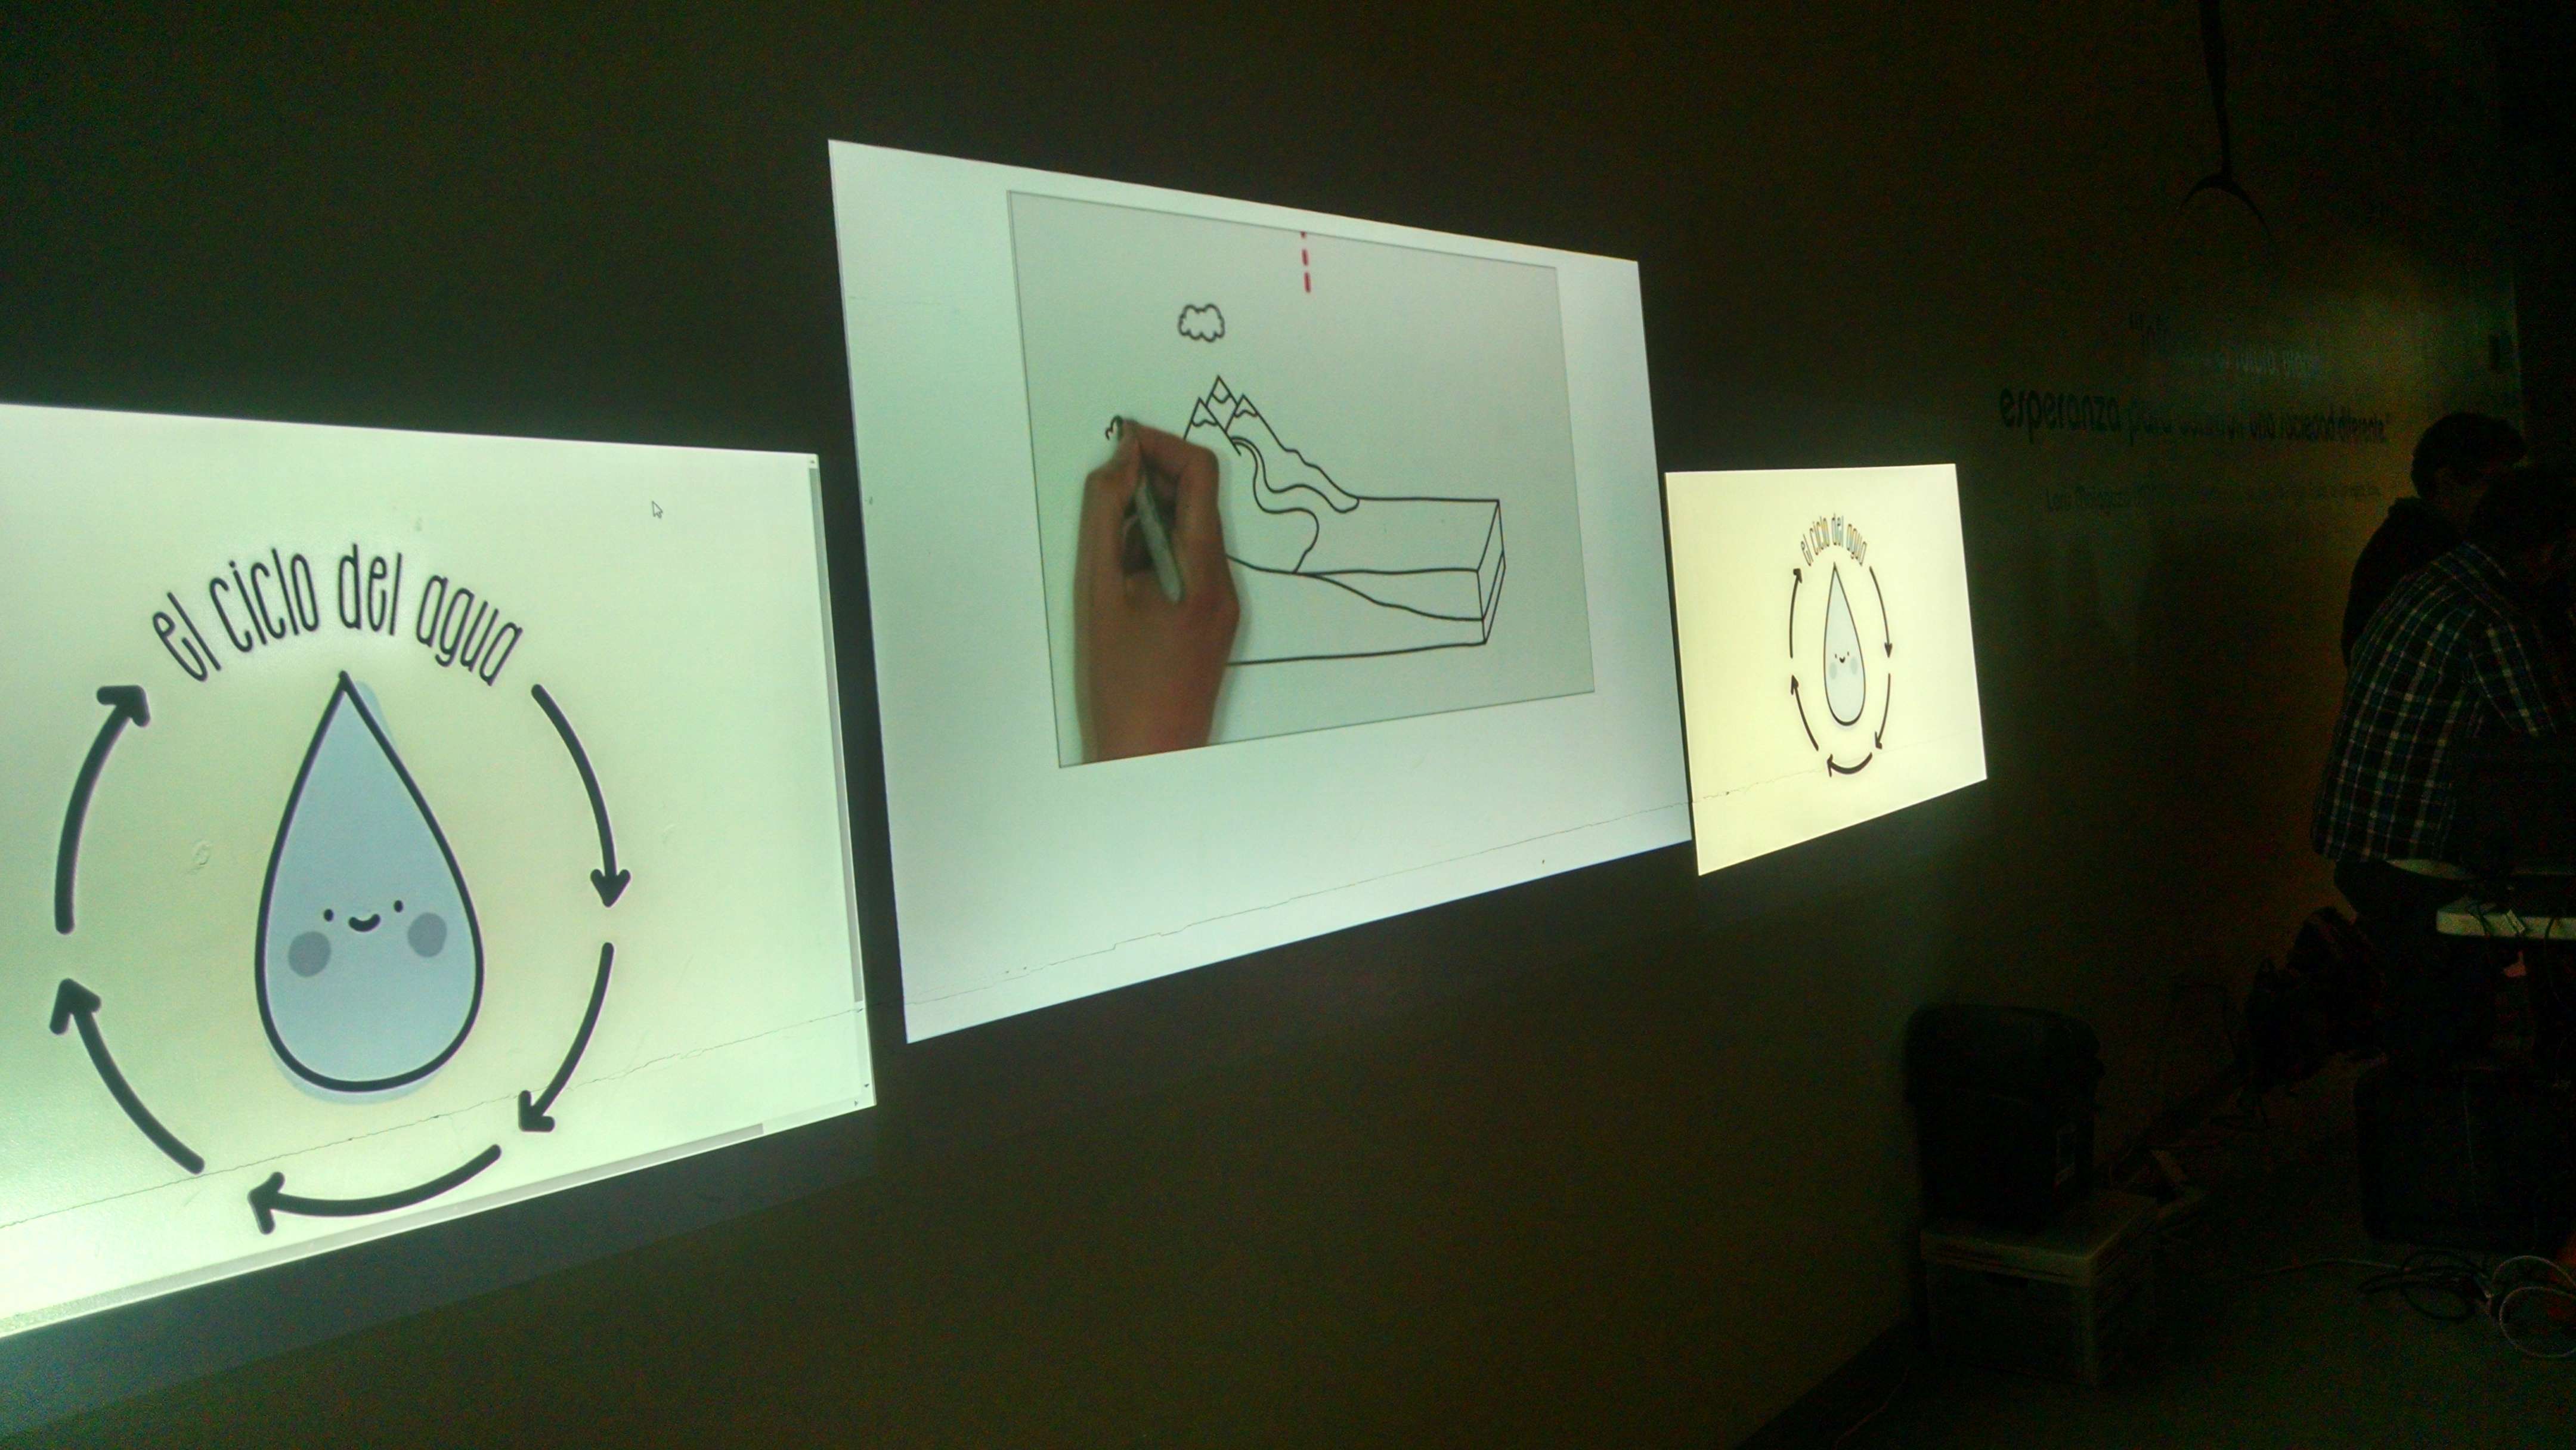
\includegraphics[scale=.08]{trompo1}
\caption{Front view of the environment.}  
\label{trompo1}  
\end{figure}
Una tablet nexus7 con la cual el usuario podia controlar la navegacion entre actividades y contestar algunos cuestionarios. y audifonos para el sonido. ademas del sensor kinekt 2 para sensar al usuario.


\subsection{Topic/Content}
Para este experimento la eleccion del tema fue influenciada por el lugar y la fecha donde se llevaria a cabo el lugar fue el museo interactivo el trompo de tijuana a pocos dias del el dia festivo "El dia del Niño" por lo que optamos por elegir un tema digerible y que haga conciencia en los usuarios. El tema elegido fue "el Cuidado del agua" donde se recabaron al rededor de 23 diferentes imagenes, 8 audios, 1 video en la figura \ref{fig:agua}. 
\begin{figure}[htbp]
\centering
\subfigure[water percent of the body]{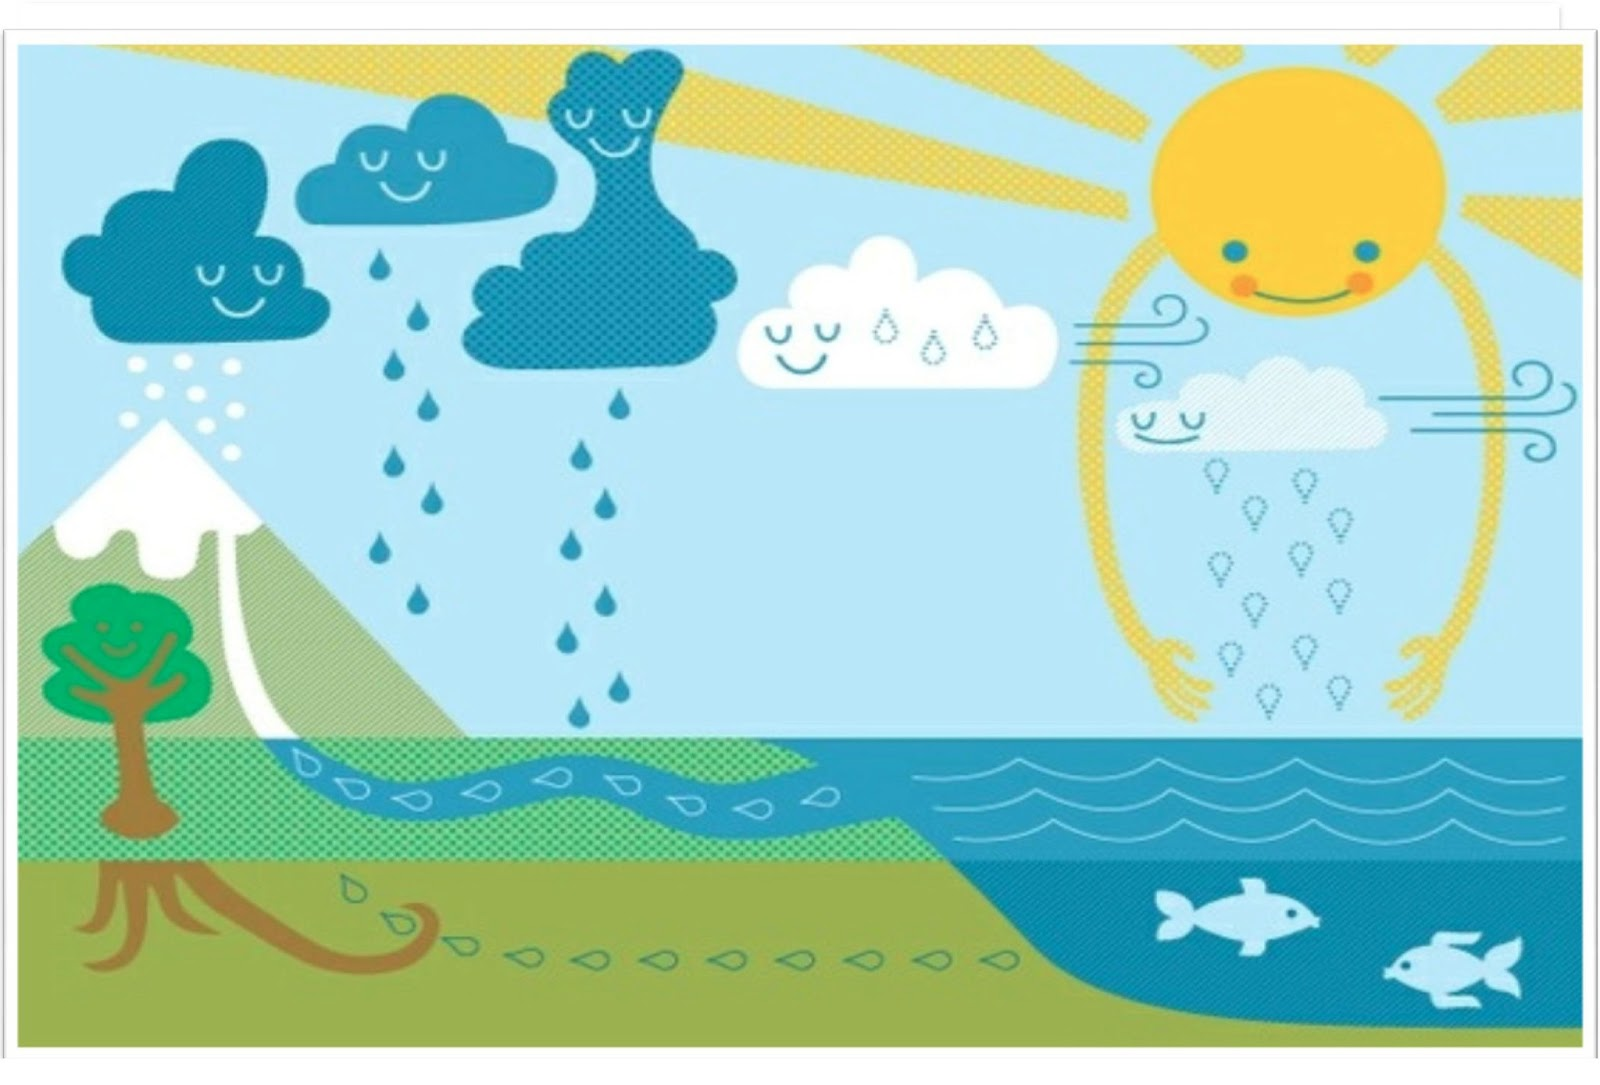
\includegraphics[width=40mm]{agua}}\hspace{10mm}
\subfigure[ciclio del agua]{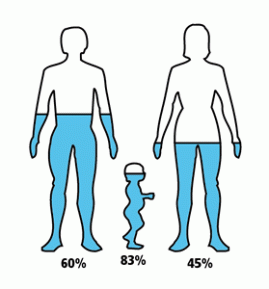
\includegraphics[width=40mm]{agua3}}\vspace{10mm}
\subfigure[total de agua en el planeta]{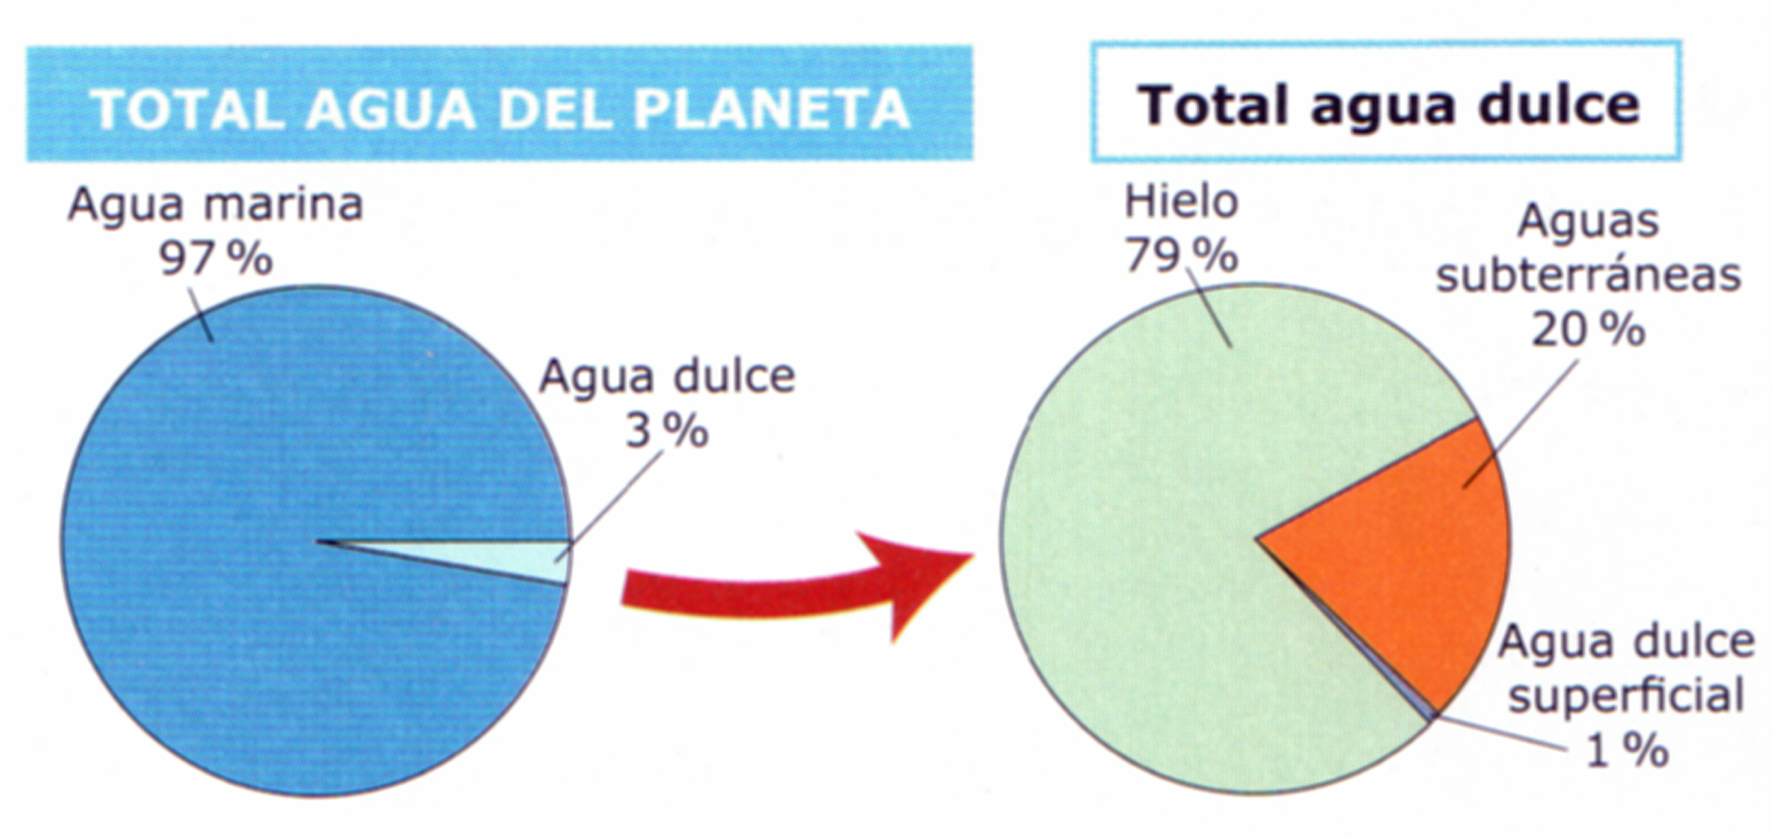
\includegraphics[width=80mm]{agua2}}
\caption{imagenes usadas en la secuencia de aprendizaje.} \label{fig:agua}
\end{figure}

La informacion mostrada por la actividad fue desde el ciclo del agua, su importacia para nuestra salud, la energia producida por la misma, ademas de el cuidado que hay que tener con ella y como evitar la contaminacion. La actividad se podia completar entre 8 y 10 minutos dependiendo de los recursos mostrados a los diferentes usuarios como lo podemos ver en la figura \ref{exp2}.

\begin{figure}[ht!]  
\centering  
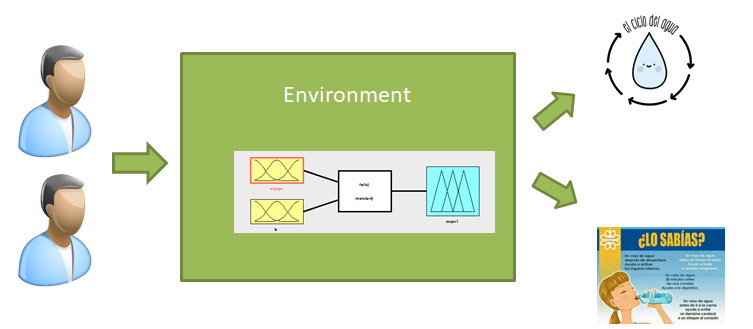
\includegraphics[scale=.5]{exp2}
\caption{How to choose content to show.}  
\label{exp2}  
\end{figure}

\subsection{Users}
This experiment was conducted with visitors of the museum’s "El trompo" where 21 users divided into 2 groups participated, the first has 10 users between 6 and 11 years 50\% men and 50\% women and the second group consisted of 11 users over 11 years old  66\% men 44\% women en la tabla \ref{tab:users21} y en la tabla \ref{tab:users22} se pueden observar algunos datos adicionales de los 2 grupos de usuarios, nota adicional algunos usuarios no quisieron revelar su edad o nombre por lo que se les respeto su desicion y se les dejo con el signo de ? y la minoria hablaba otro idioma lo que puso a prueba el contenido ya que este estaba totalmente en español aunque los usuarios aun asi participaron.
\begin{table}
\small
\centering
\captionsetup{font=footnotesize}
\caption{List of users participating in the experiment group 1.}
\label{tab:users21} 
\small
\begin{tabular}{p{3cm} p{3cm} p{3cm} }
\hline{\smallskip}
User & Name	& Age\\
\noalign{\smallskip}\hline\noalign{\smallskip}
\small{	1	}& \small{	Jose 	}& \small{	?	}\\
\small{	2	}& \small{	Mariof	}& \small{	?	}\\
\small{	3	}& \small{	Jaqueline	}& \small{	?	}\\
\small{	4	}& \small{	? 	}& \small{	10	}\\
\small{	5	}& \small{	Alondra	}& \small{	38	}\\
\small{	6	}& \small{	Josue 	}& \small{	10	}\\
\small{	7	}& \small{	Mario	}& \small{	14	}\\
\small{	8	}& \small{	Cinthya	}& \small{	30	}\\
\small{	9	}& \small{	Brisa	}& \small{	11	}\\
\small{	10	}& \small{	Hector 	}& \small{	37	}\\
\small{	11	}& \small{	Enrique	}& \small{	12	}\\
\hline
\end{tabular}
\end{table}
 
\begin{table}
\small
\centering
\captionsetup{font=footnotesize}
\caption{List of users participating in the experiment group 2.}
\label{tab:users22} 
\small
\begin{tabular}{p{3cm} p{3cm} p{3cm} }
\hline{\smallskip}
User & Name	& Age\\
\noalign{\smallskip}\hline\noalign{\smallskip}
\small{	1	}& \small{	Josue	}& \small{	8	}\\
\small{	2	}& \small{	Kevin	}& \small{	9	}\\
\small{	3	}& \small{	Monserrat	}& \small{	7	}\\
\small{	4	}& \small{	Evelin	}& \small{	9	}\\
\small{	5	}& \small{	Armando	}& \small{	8	}\\
\small{	6	}& \small{	Jorge	}& \small{	7	}\\
\small{	7	}& \small{	Gemma	}& \small{	8	}\\
\small{	8	}& \small{	Perla	}& \small{	8	}\\
\small{	9	}& \small{	Quetzal	}& \small{	7	}\\
\small{	10	}& \small{	?	}& \small{	6	}\\
\hline

\end{tabular}
\end{table}
\subsection{Survey}
Cuando los usuarios terminaron de utilizar el ambiente se les realizo una pequeña encuesta, dependiendo del usuario se le aplico una u otra encuesta que podemos observar en la tabla \ref{tab:users1} y la tabla \ref{tab:users2} respectivamente.
\begin{table}
\small
\centering
\captionsetup{font=footnotesize}
\caption{Survey to the user group 1.}
\label{tab:users2} 

\small
\begin{tabular}{p{12cm}}
\hline\noalign{\smallskip} 
Question \\
\noalign{\smallskip}\hline\noalign{\smallskip}\hline
\small{1.Did you like what you saw in the activity you just did? } \\ 

\includegraphics[width=5cm]{likert}\\ \hline  
\small{2.Did you like watching different pictures and videos? }  \\ 

\includegraphics[width=5cm]{likert}\\ \hline 
\small{3.Was it easy to use the station?  } \\ 

\includegraphics[width=5cm]{likert}\\ \hline  
\small{4.Did you have fun using the station?   } \\ 

\includegraphics[width=5cm]{likert}\\    

\hline
\noalign{\smallskip}\hline
\end{tabular}
\end{table}

\begin{table}
\small
\centering
\captionsetup{font=footnotesize}
\caption{Survey to the user group 2.}
\label{tab:users2} 

\small
\begin{tabular}{p{12cm}}
\hline\noalign{\smallskip} 
Question \\
\noalign{\smallskip}\hline\noalign{\smallskip}\hline
\small{1.I found useful for my learning this station? } \\ 
\small{	1			2			3			4			5	}\\\hline
\small{2.Using this station allowed me to learn more things faster? }  \\ 
\small{	1			2			3			4			5	}\\\hline
\small{3.The use of several images increased my understanding of the subject?  } \\ 
\small{	1			2			3			4			5	}\\\hline
\small{4.It was easy for me to use the station?   } \\ 
\small{	1			2			3			4			5	}\\\hline
\small{5.I can explain to someone how to use the station? } \\ 
\small{	1			2			3			4			5	}\\\hline
\small{6.Using this station allowed me to learn more things faster? }  \\ 
\small{	1			2			3			4			5	}\\\hline
\small{7.I think that including this station in the museum was a good idea  } \\ 
\small{	1			2			3			4			5	}\\\hline
\small{8.I liked to use the station   } \\   
\small{	1			2			3			4			5	}\\\hline
\noalign{\smallskip}\hline
\end{tabular}
\end{table}

\section{Adaptive Learning Environment topic 3}
Este experimento se llevo acabo en las instalaciones del tecnologico de tijuana ajustando nuestro prototipo con la retroalimentacion del segundo experimento. Para poder atender mas usuarios en esta ocacion las actividades fueron las mismas para todos esto permitio una mejor lectura de datos a los usuarios y minimizo el tiempo de uso de cada usuario en la actividad.This study was very similar to the last one that had some small modifications and additions, now the user no longer had control flow only observe and also to observe the user now will take video and sensor, the theme of the exhibition were video games and film as the age of the users would go for almost 17 years and older could be topics of their interest. In the same way as in the first part each user had an account to record the activity only this occasion the data produced by the sensor and videos captured by the camera would be recorded, and in the same way as in the first part at the end we surveyed the users.
For the first part of the study we get data from the survey conducted at the end, in the second they are collected and used data from sensors, this data were a bit more complex, first we need an observer to evaluate the user manually, where the observer determined whether the user was putting attention to what he saw or distracted and based on that assigned a level of attention on a scale of 1 to 3 where 1 is little attention 2 average attention and 3 very attentive. 
\subsection{Devices}
Los dispositivos usados en este experimento se describen a continuacion. Se necesito de un servidor para manejar las peticiones, almacenar los objetos de aprendizaje, generar la secuencia de aprendizaje y mantener el servicio web activo. En este caso el servidor era una computadora Mac Pro 2014 la cual cuenta con 12gb de ram y procesador intel xeon. se utilizaron 3 proyectores de las mismas resoluciones a diferentes tamaños organizados como se puede observar en la figura \ref{ambiente4}. una computadora adicional que realizo diversas tareas como mostrar el contenido de 2 proyectores y reproducir el audio,  una laptop para mostrar contenido en el tercer proyector y una laptop mas donde para obtener los datos del sensor kinect.
\begin{figure}[ht!]  
\centering  
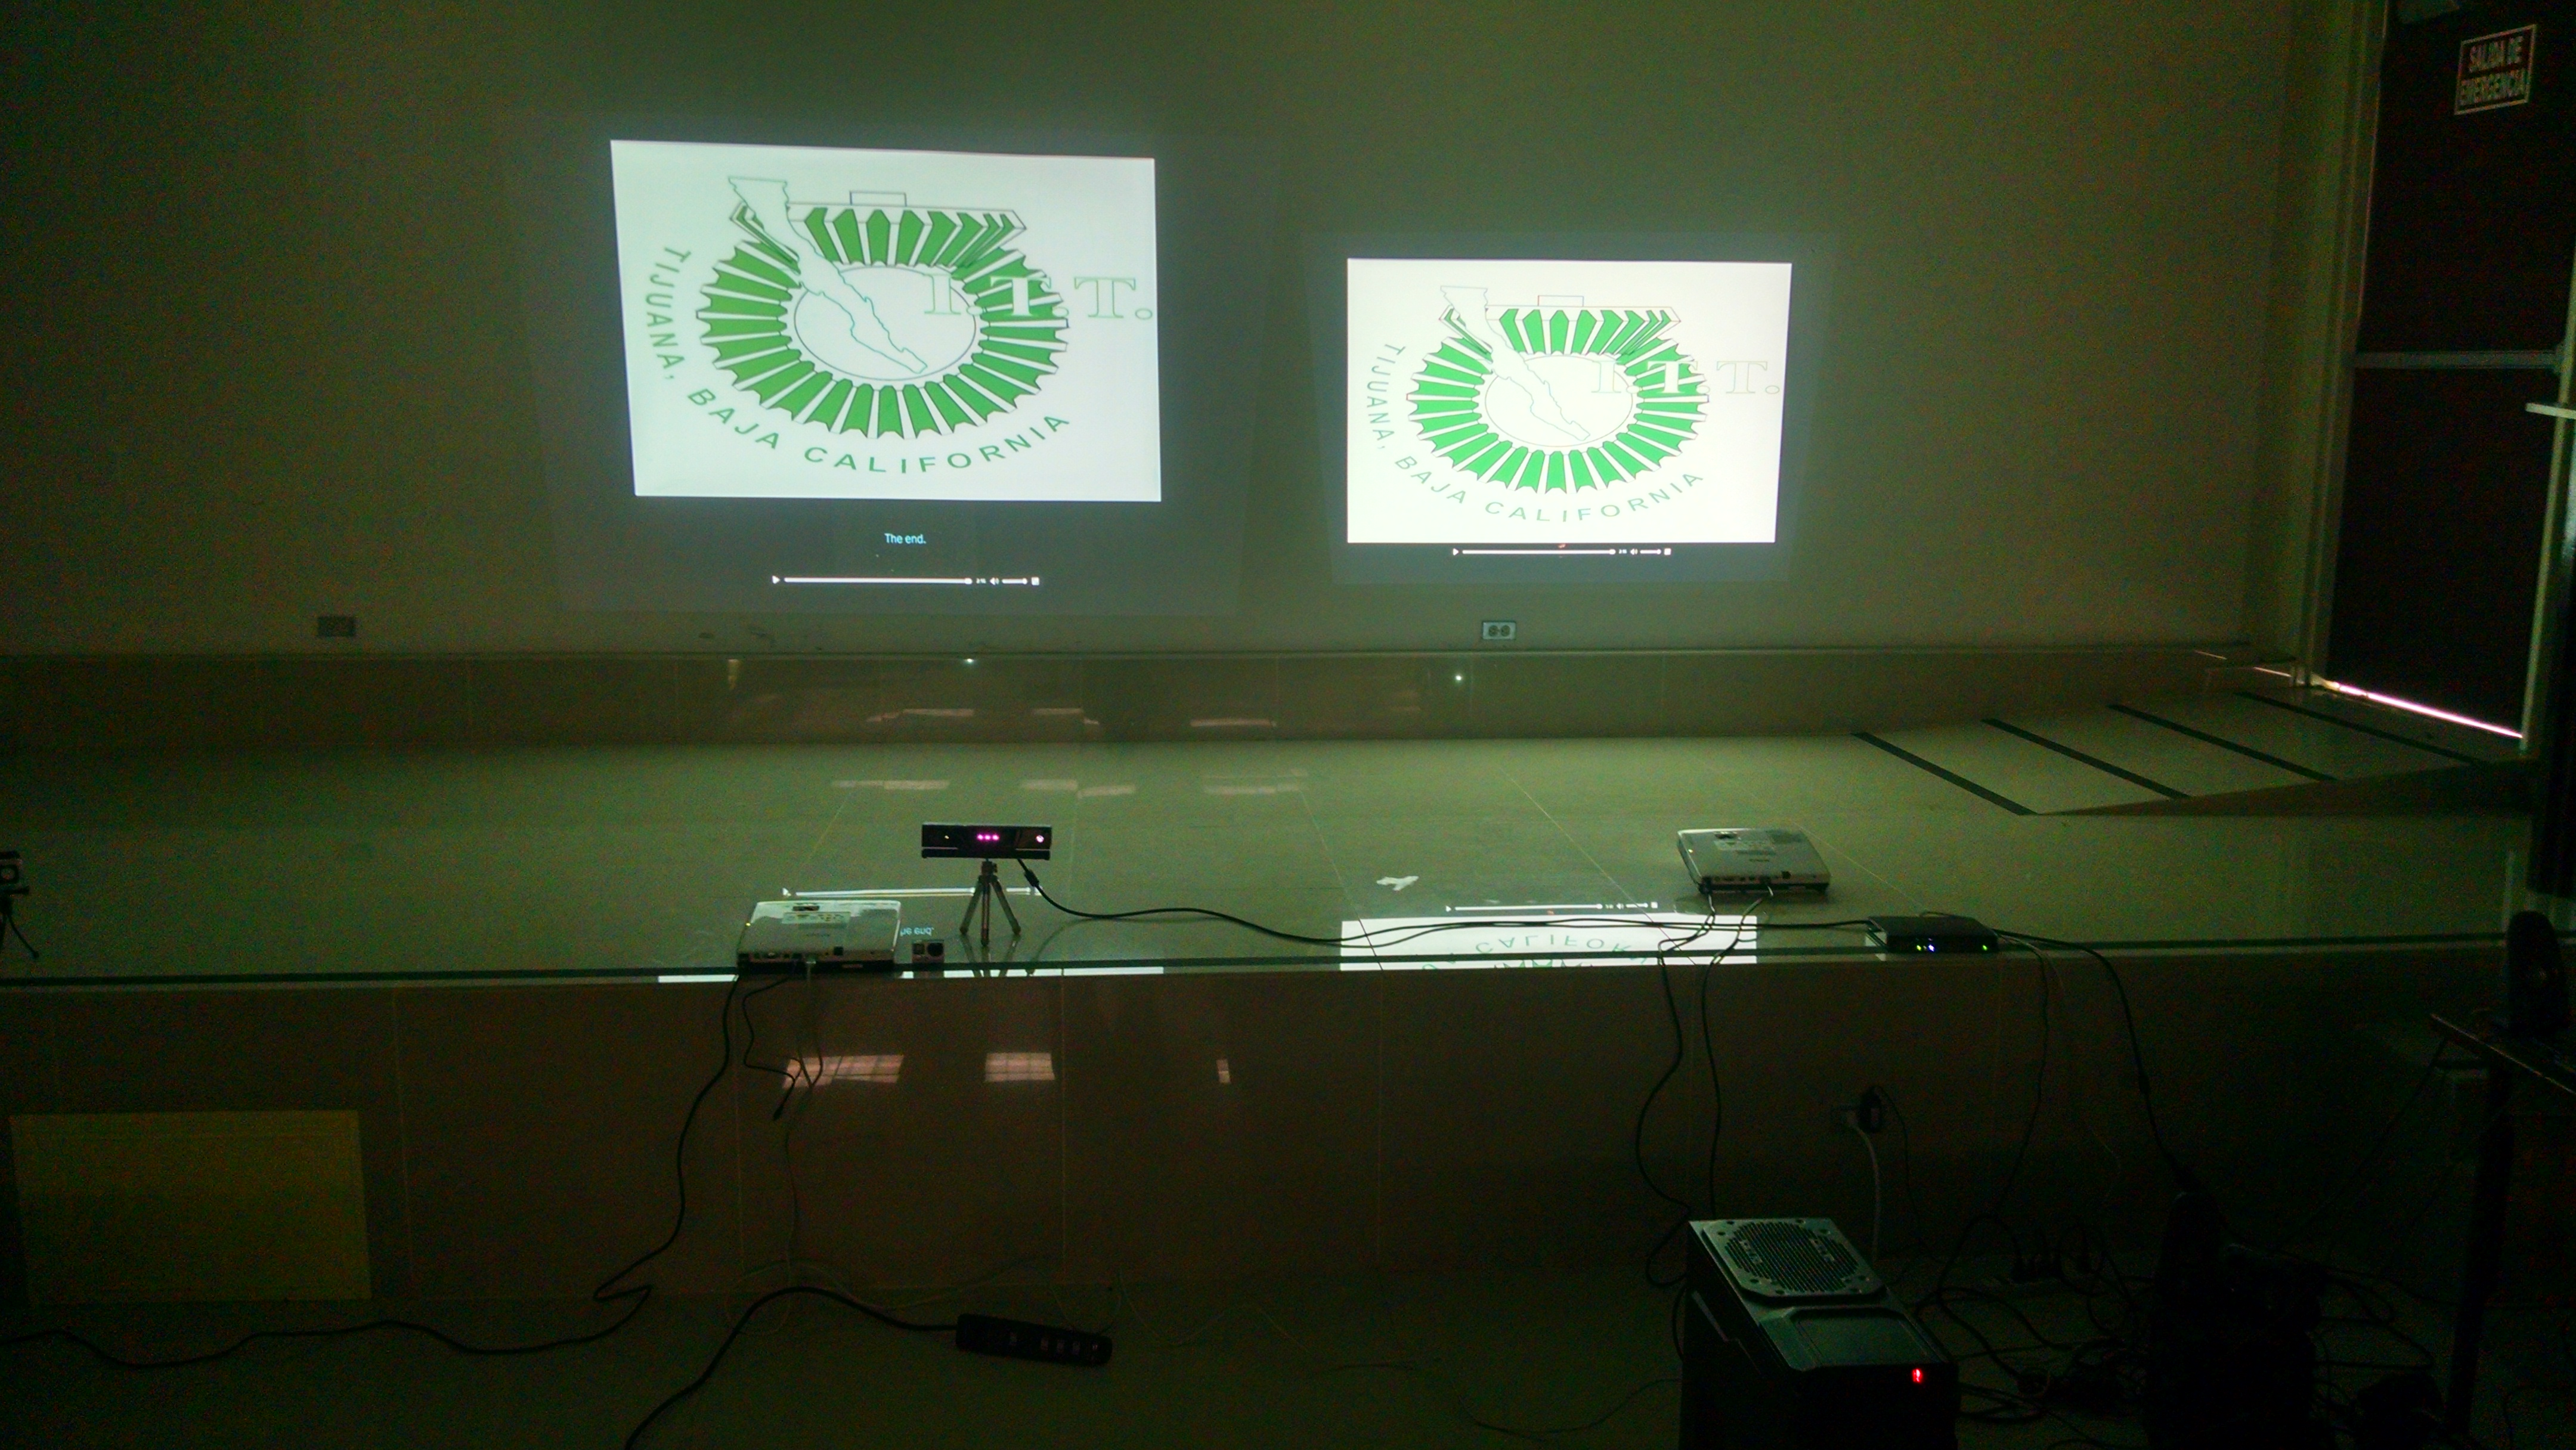
\includegraphics[scale=0.08]{tec1}
\quad  
\caption{Configuration of the last adaptive environment}  
\label{ambiente4}  
\end{figure}

\subsection{Topic/Content}
PAra elegir el tema a mostrar en el ambiente decidimos optar por temas de interez para poblacion de usuarios que fueron video juegos y el cine. el video sobre los video juegos fue sobre el video juego league of legends y el video de cine fue una explicacion de la trilogia de starwars en 2 minutos con legos.
\subsection{Users}
Participaron un total de 41 users of the Technological Institute of Tijuana were used aged between 18 and 50 years 66 \% men 34 \% women. 
\subsection{Survey}

 Cuando los usuarios terminaron de utilizar el ambiente se les realizo una pequeña encuesta que se muestra a continuacion.

\begin{table}
\small
\centering
\captionsetup{font=footnotesize}
\caption{Survey to the user group.}
\label{tab:users2} 

\small
\begin{tabular}{p{12cm}}
\hline\noalign{\smallskip} 
Age:\_\_\_\_\_\_\_\_\_\_\_\_ \\
Video 1 \\
\noalign{\smallskip}\hline\noalign{\smallskip}\hline
\small{1.How much did you like the video 1? } \\ 
\small{	1			2			3			4			5	}\\\hline
\small{2.How much did you like the main video? }  \\ 
\small{	1			2			3			4			5	}\\\hline
\small{3.How much did you like the complementary video?  } \\ 
\small{	1			2			3			4			5	}\\\hline
\hline\noalign{\smallskip} 
Video 2 \\
\noalign{\smallskip}\hline\noalign{\smallskip}\hline
\small{1.How much did you like the video 1? } \\ 
\small{	1			2			3			4			5	}\\\hline
\small{2.How much did you like the main video? }  \\ 
\small{	1			2			3			4			5	}\\\hline
\small{3.How much did you like the complementary video?  } \\
\small{	1			2			3			4			5	}\\\hline 
\hline\noalign{\smallskip} 

\small{How often do you use video games?   } \\ 
\small{	1			2			3			4			5	}\\\hline
\small{How often do you go to the cinema? } \\ 
\small{	1			2			3			4			5	}\\\hline
\hline\noalign{\smallskip} 
To play you like \\
\noalign{\smallskip}\hline\noalign{\smallskip}\hline
\small{6.Using this station allowed me to learn more things faster? }  \\ 
\small{	Phone 	1			2			3			4			5	}\\\hline
\small{	Tablet 	1			2			3			4			5	}\\\hline
\small{	PC	 	1			2			3			4			5	}\\\hline
\small{	Console		1			2			3			4			5	}\\\hline

\small{Mention 2 of your favorite video games.   } \\   
\small{		}\\\hline
\small{		}\\\hline
\small{1.How much did you like Star Wars? } \\ 
\small{	1			2			3			4			5	}\\\hline
\small{2.How much did you like Legos? }  \\ 
\small{	1			2			3			4			5	}\\\hline
\small{3.Did you like the way the information was presented?  } \\
\small{	1			2			3			4			5	}\\\hline 
\noalign{\smallskip}\hline
\end{tabular}
\end{table}




\chapter{Environment Evaluation} \label{enveva} 
\chapter{Conclutions} \label{conclu} 
%En este trabajo de investigaci�n, se desarrollo un ambiente de aprendizaje interactivo con m�ltiples usos como exhibidor de museo, entretenimiento, publicidad, etc. La principal caracter�stica de este ambiente de aprendizaje es que cuenta con un objeto de aprendizaje especial que al combinarse con el ambiente le permite ser lo que se mencionaba antes.
%El desempe�o de este ambiente lo medimos en varias pruebas con usuarios reales, el ambiente en sus primeras versiones fue probado con usuarios �locales� (Usuarios al alcance del laboratorio) para medir la aceptaci�n de este tipo de tecnolog�a y que tan f�cil era de utilizar el ambiente en la cual tuvimos buenos resultados.
In this research work, an interactive learning environment was developed with multiple uses as a museum exhibitor, entertainment, advertising, etc. The main feature of this learning environment is that it has a special learning object that when combined with the environment allows it to be what was mentioned before.
The performance of this environment is measured in several tests with real users, the environment in its early versions was tested with "local users" (Users within the scope of the laboratory) to measure the acceptance of this type of technology and how easy it was to use The environment in which we had good results.
 
%En la segunda versi�n nos trasladamos al museo interactivo de Tijuana El trompo donde el objetivo de la prueba fue usarlo con usuarios de diversas edades y observar las reacciones de estos mismos desde esta versi�n utilizamos el sensor de Kinect 2 para observar el usuario pero la informaci�n obtenida no fue lo suficientemente buena para utilizarla, en esta ocasi�n el ambiente con informaci�n dada por el usuario era capaz de modificar la informaci�n mostrada en un intento por adaptar la informaci�n y ser m�s atractiva para el usuario. Al no poder utilizar la informaci�n dada por el sensor optamos por conservar las encuestas que les aplicamos a los usuarios las cuales mostraron muy buena aceptaci�n en su mayor�a, los pocos que no estuvieron de acuerdo fueron ni�os menores de 6 a�os los cuales mostraron poco inter�s y un nivel de distracci�n un poco alto esto lo atribuimos a que los ni�os eran extranjeros y no dominaban muy poco idioma espa�ol que era el idioma que manejaba el ambiente. 
In the second version we moved to the interactive museum in Tijuana The spinning wheel where the objective of the test was to use it with users of different ages and to observe the reactions of these same ones from this version we used the sensor of Kinect 2 to observe the user but the obtained information Was not good enough to use it, this time the environment with information given by the user was able to modify the information shown in an attempt to adapt the information and be more attractive to the user. When we could not use the information given by the sensor we chose to keep the surveys we applied to the users, which showed very good acceptance in the majority, the few who did not agree were children under 6 years old who showed little interest and A level of distraction a little high we attribute this to the children were foreigners and did not have very little Spanish language that was the language that managed the environment.  

%En la �ltima versi�n del ambiente fue utilizado en el instituto tecnol�gico de Tijuana utilizando un grupo de usuarios m�s homog�neo los cuales eran alumnos y algunos maestros de la escuela, en esta prueba los usuarios adem�s de ser observados por el sensor tambi�n se les tomo video para analizarlo y tener una referencia para los resultados de la clasificaci�n de datos dada por el sensor adem�s se le aplico una encuesta a los usuarios para identificar los gustos en cuanto a informaci�n y los dispositivos que utilizan los usuarios. cada una de las pruebas el ambiente evolucionaba gracias a la informaci�n proporcionada por los usuarios de ir de algo muy simple como solo mostrar im�genes a mostrar videos, reproducir audios. Luego de ciertas modificaciones pudimos manipular contenido y secuenciarlo.
In the last version of the environment was used in the technological institute of Tijuana using a more homogeneous group of users who were students and some teachers of the school, in this test users in addition to being observed by the sensor were also taken video for Analyze it and have a reference for the results of the classification of data given by the sensor also applied a survey to users to identify the tastes in terms of information and devices used by users. Each of the tests the environment evolved thanks to the information provided by users to go from something very simple like just showing pictures to show videos, play audio. After some modifications we were able to manipulate content and sequence it.


\appendix
%% Cap'itulos incluidos despues del comando \appendix aparecen como ap'endices
%% de la tesis.
%\include{apendiceA}
%\include{apendiceB}
%\include{apendiceC}

\bibliography{biblio}
%% Incluir la bibliograf'ia. Mirar el archivo "biblio.bib" para m'as detales
%% y un ejemplo.


\end{document}
